\chapter{Tidal Disruption of Neutron Stars with New Nuclear Equations of State}
\label{chap:chapter-5}

\textbf{TODO: Much more analysis to be done...}

\begin{table}
	\begin{center}
	\caption[Initial parameters of binaries used in this survey]{
		Initial parameters of the binaries studied in this paper. 
		$M_{\rm NS}$ the ADM mass of an isolated neutron star with the same equation of state and baryon mass as the neutron star under
		consideration, $N_{\rm orbits}$ is the number of orbits up to the point at which $0.01M_\odot$ has been accreted by the black hole,
		$\Omega_0$ is the initial angular velocity, and $M=M_{\rm BH}+M_{\rm NS}$. We use the same resolution for each simulation: $\Delta x_{\rm dis} = 245{\rm m}$ is the typical grid resolution in the laboratory frame
		for the finest level of refinement used during the disruption of the neutron star (see Sec.~\ref{sec:hydro-amr} for more detail on the grid structure).}
	\label{tab:id}
	{
		\begin{tabular}{|l||ccccc|}
	%\toprule
	\hline
	Model & $M_{\rm NS}\,(M_\odot)$ & $R_{\rm NS}\,({\rm km})$ & $\cal{C}_{\rm NS}$ & $N_{\rm orbits}$ & $\Omega_0 M$ \\
	%\midrule\midrule
	\hline%\hline
	M12-M7-S9-DD2 & 1.2 & 13.1 & 0.135 & 5.0 & fill1\\
	M14-M7-S9-DD2 & 1.4 & 13.2 & 0.156 & 6.0 & fill1\\
	M12-M7-S9-FSU21 & 1.2 & 13.5 & 0.130 & 4.9 & fill1\\
	M14-M7-S9-FSU21 & 1.4 & 13.6 & 0.152 & 5.5 & fill1\\
	M12-M7-S9-SFHo & 1.2 & 11.9 & 0.148 & 5.3 & fill1\\
	M14-M7-S9-SFHo & 1.4 & 11.8 & 0.173 & 5.9 & fill1\\
	M12-M7-S9-SFHx & 1.2 & 11.9 & 0.149 & 5.2 & fill1\\
	M14-M7-S9-SFHx & 1.4 & 11.9 & 0.173 & 5.4 & fill1\\
%			M12-M7-S9-LS220 & 1.2 & 12.7 & 0.139 & fill0 & fill & 160\\
%			M14-M7-S9-LS220 & 1.4 & 12.6 & 0.163 & fill0 & fill & 170\\
	\hline
	%\bottomrule
\end{tabular}
	}
	\end{center}
\end{table}

\begin{table}
	\begin{center}
	\caption[Properties of the dynamical ejecta and post merger remnant]{
		Properties of the dynamical ejecta and post merger remnant. $M_{\rm BH}^f$ and  $\chi_{\rm BH}^f$  are the mass and dimensionless spin of the black hole,
		and $M_{\rm out}^f$ is the baryon mass remaining outside of the black hole. Those quantities are measured at the first minima of the accretion rate onto the black hole,
		before circularization of the accretion disk. The baryon mass outside of the black hole immediately after disk formation (which is a more vaguely defined
		time) is typically $10\%-20\%$ lower than $M_{\rm out}^f$. $M_{\rm ej}$ is the mass of the dynamical ejecta, and $\langle v/c\rangle_{\rm ej}$, 
		$\langle i \rangle_{\rm ej}$ are the mass-weighted average of its velocity and orbital inclination with respect to the
		equatorial plane of the black hole. All these properties are nearly constant, from about $1\,{\rm ms}$ after the merger. Bracketed numbers for
		$M_{\rm out}^f$ and $M_{\rm ej}$ show semi-analytical predictions for the mass outside of the black hole $10\,{\rm ms}$ after merger~\cite{Foucart2012},
		and the ejected mass~\cite{Kawaguchi:2016}, while bracketed numbers for $M_{\rm BH}^f$ and $\chi_{\rm BH}^f$ are semi-analytical predictions
		from~\cite{Pannarale:2014}. The analytical values provided in this table for the final mass and spin of the black hole were kindly provided
		to us by Francesco Pannarale. Relative errors in the determination of $M_{\rm ej}$ are $\sim 20\%$, the black holes properties are
		accurate to $\sim 1\%$, and other quantities have relative errors of $\sim 10\%$.
	}
	\label{tab:results}
	{
		\begin{tabular}{c cc ccc}
	\toprule \toprule
	Model & $M_{\rm BH}^f\,(M_\odot)$ & $\chi_{\rm BH}^f$ & $M_{\rm out}^f\,(10^{-2} M_\odot)$ & $M_{\rm ej}\,(10^{-2} M_\odot)$ & $\langle v/c \rangle_{\rm ej}$\\
	\midrule
	M12-M7-S9-DD2 & -- [7.7] & -- [0.93] & -- [36] & 7.2 [7.2] & 0.21\\
	M14-M7-S9-DD2 & -- [7.9] & -- [0.93] & -- [34] & 6.0 [3.6] & 0.20\\
	M12-M7-S9-FSU21 & -- [7.7] & -- [0.93] & -- [38] & 7.8 [10.7] & 0.20\\
	M14-M7-S9-FSU21 & -- [7.9] & -- [0.93] & -- [36] & 5.9 [6.4] & 0.19\\
	M12-M7-S9-SFHo & -- [7.8] & -- [0.93] & -- [30] & $\sym 3.8$ [4.3] & $\sym 0.18$\\
	M14-M7-S9-SFHo & -- [8.0] & -- [0.93] & -- [26] & -- [2.3] & --\\
	M12-M7-S9-SFHx & -- [7.8] & -- [0.93] & -- [30] & $\sym 5.7$ [5.9] & $\sym0.20 $\\
	M14-M7-S9-SFHx & -- [8.0] & -- [0.93] & -- [26] & -- [2.6] & --\\
%	M12-M7-S9-LS220 & -- [7.8] & -- [0.93] & -- [34] & -- [9.4] & --\\
%	M14-M7-S9-LS220 & -- [8.0] & -- [0.93] & -- [31] & -- [4.7] & --\\
	\bottomrule \bottomrule
\end{tabular}
	}
	\end{center}
\end{table}



\begin{figure}
	\centering
	% GNUPLOT: LaTeX picture with Postscript
\begingroup
  \makeatletter
  \providecommand\color[2][]{%
    \GenericError{(gnuplot) \space\space\space\@spaces}{%
      Package color not loaded in conjunction with
      terminal option `colourtext'%
    }{See the gnuplot documentation for explanation.%
    }{Either use 'blacktext' in gnuplot or load the package
      color.sty in LaTeX.}%
    \renewcommand\color[2][]{}%
  }%
  \providecommand\includegraphics[2][]{%
    \GenericError{(gnuplot) \space\space\space\@spaces}{%
      Package graphicx or graphics not loaded%
    }{See the gnuplot documentation for explanation.%
    }{The gnuplot epslatex terminal needs graphicx.sty or graphics.sty.}%
    \renewcommand\includegraphics[2][]{}%
  }%
  \providecommand\rotatebox[2]{#2}%
  \@ifundefined{ifGPcolor}{%
    \newif\ifGPcolor
    \GPcolortrue
  }{}%
  \@ifundefined{ifGPblacktext}{%
    \newif\ifGPblacktext
    \GPblacktexttrue
  }{}%
  % define a \g@addto@macro without @ in the name:
  \let\gplgaddtomacro\g@addto@macro
  % define empty templates for all commands taking text:
  \gdef\gplbacktext{}%
  \gdef\gplfronttext{}%
  \makeatother
  \ifGPblacktext
    % no textcolor at all
    \def\colorrgb#1{}%
    \def\colorgray#1{}%
  \else
    % gray or color?
    \ifGPcolor
      \def\colorrgb#1{\color[rgb]{#1}}%
      \def\colorgray#1{\color[gray]{#1}}%
      \expandafter\def\csname LTw\endcsname{\color{white}}%
      \expandafter\def\csname LTb\endcsname{\color{black}}%
      \expandafter\def\csname LTa\endcsname{\color{black}}%
      \expandafter\def\csname LT0\endcsname{\color[rgb]{1,0,0}}%
      \expandafter\def\csname LT1\endcsname{\color[rgb]{0,1,0}}%
      \expandafter\def\csname LT2\endcsname{\color[rgb]{0,0,1}}%
      \expandafter\def\csname LT3\endcsname{\color[rgb]{1,0,1}}%
      \expandafter\def\csname LT4\endcsname{\color[rgb]{0,1,1}}%
      \expandafter\def\csname LT5\endcsname{\color[rgb]{1,1,0}}%
      \expandafter\def\csname LT6\endcsname{\color[rgb]{0,0,0}}%
      \expandafter\def\csname LT7\endcsname{\color[rgb]{1,0.3,0}}%
      \expandafter\def\csname LT8\endcsname{\color[rgb]{0.5,0.5,0.5}}%
    \else
      % gray
      \def\colorrgb#1{\color{black}}%
      \def\colorgray#1{\color[gray]{#1}}%
      \expandafter\def\csname LTw\endcsname{\color{white}}%
      \expandafter\def\csname LTb\endcsname{\color{black}}%
      \expandafter\def\csname LTa\endcsname{\color{black}}%
      \expandafter\def\csname LT0\endcsname{\color{black}}%
      \expandafter\def\csname LT1\endcsname{\color{black}}%
      \expandafter\def\csname LT2\endcsname{\color{black}}%
      \expandafter\def\csname LT3\endcsname{\color{black}}%
      \expandafter\def\csname LT4\endcsname{\color{black}}%
      \expandafter\def\csname LT5\endcsname{\color{black}}%
      \expandafter\def\csname LT6\endcsname{\color{black}}%
      \expandafter\def\csname LT7\endcsname{\color{black}}%
      \expandafter\def\csname LT8\endcsname{\color{black}}%
    \fi
  \fi
  \setlength{\unitlength}{0.0500bp}%
  \begin{picture}(7200.00,5040.00)%
    \gplgaddtomacro\gplbacktext{%
      \csname LTb\endcsname%
      \put(946,704){\makebox(0,0)[r]{\strut{} 0.4}}%
      \put(946,1317){\makebox(0,0)[r]{\strut{} 0.6}}%
      \put(946,1929){\makebox(0,0)[r]{\strut{} 0.8}}%
      \put(946,2542){\makebox(0,0)[r]{\strut{} 1}}%
      \put(946,3154){\makebox(0,0)[r]{\strut{} 1.2}}%
      \put(946,3766){\makebox(0,0)[r]{\strut{} 1.4}}%
      \put(946,4379){\makebox(0,0)[r]{\strut{} 1.6}}%
      \put(1078,484){\makebox(0,0){\strut{} 2}}%
      \put(1896,484){\makebox(0,0){\strut{} 3}}%
      \put(2714,484){\makebox(0,0){\strut{} 4}}%
      \put(3532,484){\makebox(0,0){\strut{} 5}}%
      \put(4349,484){\makebox(0,0){\strut{} 6}}%
      \put(5167,484){\makebox(0,0){\strut{} 7}}%
      \put(5985,484){\makebox(0,0){\strut{} 8}}%
      \put(6803,484){\makebox(0,0){\strut{} 9}}%
      \put(176,2541){\rotatebox{-270}{\makebox(0,0){\strut{}$M^b_{\rm NS}$ ($M_{\odot}$)}}}%
      \put(3940,154){\makebox(0,0){\strut{}$t - t_{\rm plunge}$ (ms)}}%
      \put(3940,4709){\makebox(0,0){\strut{}Neutron star mass in plunge-merger for hot Nuclear-theory EOSs}}%
    }%
    \gplgaddtomacro\gplfronttext{%
      \csname LTb\endcsname%
      \put(5816,4206){\makebox(0,0)[r]{\strut{}Hempel DD2 M=1.2}}%
      \csname LTb\endcsname%
      \put(5816,3986){\makebox(0,0)[r]{\strut{}Hempel DD2 M=1.4}}%
      \csname LTb\endcsname%
      \put(5816,3766){\makebox(0,0)[r]{\strut{}G. Shen FSU 2.1, M=1.2}}%
      \csname LTb\endcsname%
      \put(5816,3546){\makebox(0,0)[r]{\strut{}G. Shen FSU 2.1, M=1.4}}%
      \csname LTb\endcsname%
      \put(5816,3326){\makebox(0,0)[r]{\strut{}SettleDisk}}%
      \csname LTb\endcsname%
      \put(5816,3106){\makebox(0,0)[r]{\strut{}Derefinement 1}}%
      \csname LTb\endcsname%
      \put(5816,2886){\makebox(0,0)[r]{\strut{}Derefinement 2}}%
      \csname LTb\endcsname%
      \put(5816,2666){\makebox(0,0)[r]{\strut{}Adaptive JB}}%
      \csname LTb\endcsname%
      \put(5816,2446){\makebox(0,0)[r]{\strut{}SFHo M=1.2}}%
      \csname LTb\endcsname%
      \put(5816,2226){\makebox(0,0)[r]{\strut{}SFHo M=1.4}}%
      \csname LTb\endcsname%
      \put(5816,2006){\makebox(0,0)[r]{\strut{}SFHx M=1.2}}%
      \csname LTb\endcsname%
      \put(5816,1786){\makebox(0,0)[r]{\strut{}SFHx M=1.4}}%
    }%
    \gplbacktext
    \put(0,0){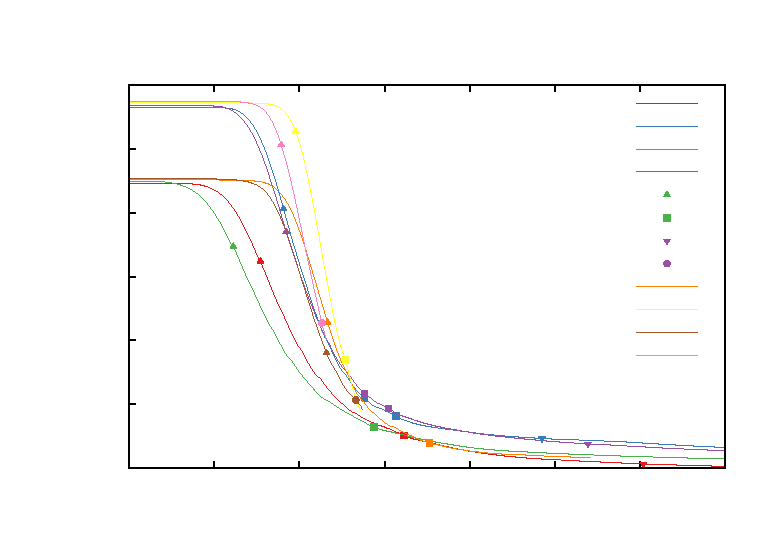
\includegraphics{images/combined-restmass}}%
    \gplfronttext
  \end{picture}%
\endgroup

	\caption[]{
		\textbf{TODO}
	}
	\label{fig:restmass}
\end{figure}

\begin{figure}
	\centering
	% GNUPLOT: LaTeX picture with Postscript
\begingroup
  \makeatletter
  \providecommand\color[2][]{%
    \GenericError{(gnuplot) \space\space\space\@spaces}{%
      Package color not loaded in conjunction with
      terminal option `colourtext'%
    }{See the gnuplot documentation for explanation.%
    }{Either use 'blacktext' in gnuplot or load the package
      color.sty in LaTeX.}%
    \renewcommand\color[2][]{}%
  }%
  \providecommand\includegraphics[2][]{%
    \GenericError{(gnuplot) \space\space\space\@spaces}{%
      Package graphicx or graphics not loaded%
    }{See the gnuplot documentation for explanation.%
    }{The gnuplot epslatex terminal needs graphicx.sty or graphics.sty.}%
    \renewcommand\includegraphics[2][]{}%
  }%
  \providecommand\rotatebox[2]{#2}%
  \@ifundefined{ifGPcolor}{%
    \newif\ifGPcolor
    \GPcolortrue
  }{}%
  \@ifundefined{ifGPblacktext}{%
    \newif\ifGPblacktext
    \GPblacktexttrue
  }{}%
  % define a \g@addto@macro without @ in the name:
  \let\gplgaddtomacro\g@addto@macro
  % define empty templates for all commands taking text:
  \gdef\gplbacktext{}%
  \gdef\gplfronttext{}%
  \makeatother
  \ifGPblacktext
    % no textcolor at all
    \def\colorrgb#1{}%
    \def\colorgray#1{}%
  \else
    % gray or color?
    \ifGPcolor
      \def\colorrgb#1{\color[rgb]{#1}}%
      \def\colorgray#1{\color[gray]{#1}}%
      \expandafter\def\csname LTw\endcsname{\color{white}}%
      \expandafter\def\csname LTb\endcsname{\color{black}}%
      \expandafter\def\csname LTa\endcsname{\color{black}}%
      \expandafter\def\csname LT0\endcsname{\color[rgb]{1,0,0}}%
      \expandafter\def\csname LT1\endcsname{\color[rgb]{0,1,0}}%
      \expandafter\def\csname LT2\endcsname{\color[rgb]{0,0,1}}%
      \expandafter\def\csname LT3\endcsname{\color[rgb]{1,0,1}}%
      \expandafter\def\csname LT4\endcsname{\color[rgb]{0,1,1}}%
      \expandafter\def\csname LT5\endcsname{\color[rgb]{1,1,0}}%
      \expandafter\def\csname LT6\endcsname{\color[rgb]{0,0,0}}%
      \expandafter\def\csname LT7\endcsname{\color[rgb]{1,0.3,0}}%
      \expandafter\def\csname LT8\endcsname{\color[rgb]{0.5,0.5,0.5}}%
    \else
      % gray
      \def\colorrgb#1{\color{black}}%
      \def\colorgray#1{\color[gray]{#1}}%
      \expandafter\def\csname LTw\endcsname{\color{white}}%
      \expandafter\def\csname LTb\endcsname{\color{black}}%
      \expandafter\def\csname LTa\endcsname{\color{black}}%
      \expandafter\def\csname LT0\endcsname{\color{black}}%
      \expandafter\def\csname LT1\endcsname{\color{black}}%
      \expandafter\def\csname LT2\endcsname{\color{black}}%
      \expandafter\def\csname LT3\endcsname{\color{black}}%
      \expandafter\def\csname LT4\endcsname{\color{black}}%
      \expandafter\def\csname LT5\endcsname{\color{black}}%
      \expandafter\def\csname LT6\endcsname{\color{black}}%
      \expandafter\def\csname LT7\endcsname{\color{black}}%
      \expandafter\def\csname LT8\endcsname{\color{black}}%
    \fi
  \fi
  \setlength{\unitlength}{0.0500bp}%
  \begin{picture}(7200.00,5040.00)%
    \gplgaddtomacro\gplbacktext{%
      \csname LTb\endcsname%
      \put(814,704){\makebox(0,0)[r]{\strut{} 0}}%
      \put(814,1439){\makebox(0,0)[r]{\strut{} 5}}%
      \put(814,2174){\makebox(0,0)[r]{\strut{} 10}}%
      \put(814,2909){\makebox(0,0)[r]{\strut{} 15}}%
      \put(814,3644){\makebox(0,0)[r]{\strut{} 20}}%
      \put(814,4379){\makebox(0,0)[r]{\strut{} 25}}%
      \put(946,484){\makebox(0,0){\strut{} 0}}%
      \put(1783,484){\makebox(0,0){\strut{} 2}}%
      \put(2619,484){\makebox(0,0){\strut{} 4}}%
      \put(3456,484){\makebox(0,0){\strut{} 6}}%
      \put(4293,484){\makebox(0,0){\strut{} 8}}%
      \put(5130,484){\makebox(0,0){\strut{} 10}}%
      \put(5966,484){\makebox(0,0){\strut{} 12}}%
      \put(6803,484){\makebox(0,0){\strut{} 14}}%
      \put(176,2541){\rotatebox{-270}{\makebox(0,0){\strut{}$\langle T \rangle$ (MeV)}}}%
      \put(3874,154){\makebox(0,0){\strut{}$t - t_{\rm settledisk}$ (ms)}}%
      \put(3874,4709){\makebox(0,0){\strut{}Average Temperatures in merger for hot Nuclear-theory EOSs}}%
    }%
    \gplgaddtomacro\gplfronttext{%
      \csname LTb\endcsname%
      \put(1933,3077){\makebox(0,0)[l]{\strut{}Hempel DD2 M=1.2}}%
      \csname LTb\endcsname%
      \put(1933,2857){\makebox(0,0)[l]{\strut{}Hempel DD2 M=1.4}}%
      \csname LTb\endcsname%
      \put(1933,2637){\makebox(0,0)[l]{\strut{}G. Shen FSU 2.1, M=1.2}}%
      \csname LTb\endcsname%
      \put(1933,2417){\makebox(0,0)[l]{\strut{}G. Shen FSU 2.1, M=1.4}}%
      \csname LTb\endcsname%
      \put(1933,2197){\makebox(0,0)[l]{\strut{}Derefinement 1}}%
      \csname LTb\endcsname%
      \put(1933,1977){\makebox(0,0)[l]{\strut{}Derefinement 2}}%
      \csname LTb\endcsname%
      \put(1933,1757){\makebox(0,0)[l]{\strut{}Adaptive JB}}%
      \csname LTb\endcsname%
      \put(1933,1537){\makebox(0,0)[l]{\strut{}SFHo M=1.2}}%
      \csname LTb\endcsname%
      \put(1933,1317){\makebox(0,0)[l]{\strut{}SFHo M=1.4}}%
      \csname LTb\endcsname%
      \put(1933,1097){\makebox(0,0)[l]{\strut{}SFHx M=1.2}}%
      \csname LTb\endcsname%
      \put(1933,877){\makebox(0,0)[l]{\strut{}SFHx M=1.4}}%
    }%
    \gplbacktext
    \put(0,0){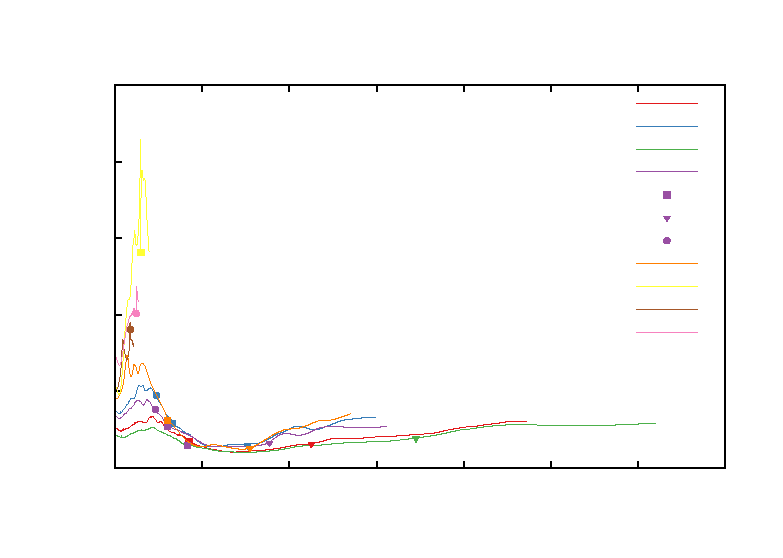
\includegraphics{images/combined-average-temp}}%
    \gplfronttext
  \end{picture}%
\endgroup

	\caption[]{
		\textbf{TODO}
	}
	\label{fig:avgtemp}
\end{figure}

\begin{figure}
	\centering
	% GNUPLOT: LaTeX picture with Postscript
\begingroup
  \makeatletter
  \providecommand\color[2][]{%
    \GenericError{(gnuplot) \space\space\space\@spaces}{%
      Package color not loaded in conjunction with
      terminal option `colourtext'%
    }{See the gnuplot documentation for explanation.%
    }{Either use 'blacktext' in gnuplot or load the package
      color.sty in LaTeX.}%
    \renewcommand\color[2][]{}%
  }%
  \providecommand\includegraphics[2][]{%
    \GenericError{(gnuplot) \space\space\space\@spaces}{%
      Package graphicx or graphics not loaded%
    }{See the gnuplot documentation for explanation.%
    }{The gnuplot epslatex terminal needs graphicx.sty or graphics.sty.}%
    \renewcommand\includegraphics[2][]{}%
  }%
  \providecommand\rotatebox[2]{#2}%
  \@ifundefined{ifGPcolor}{%
    \newif\ifGPcolor
    \GPcolortrue
  }{}%
  \@ifundefined{ifGPblacktext}{%
    \newif\ifGPblacktext
    \GPblacktexttrue
  }{}%
  % define a \g@addto@macro without @ in the name:
  \let\gplgaddtomacro\g@addto@macro
  % define empty templates for all commands taking text:
  \gdef\gplbacktext{}%
  \gdef\gplfronttext{}%
  \makeatother
  \ifGPblacktext
    % no textcolor at all
    \def\colorrgb#1{}%
    \def\colorgray#1{}%
  \else
    % gray or color?
    \ifGPcolor
      \def\colorrgb#1{\color[rgb]{#1}}%
      \def\colorgray#1{\color[gray]{#1}}%
      \expandafter\def\csname LTw\endcsname{\color{white}}%
      \expandafter\def\csname LTb\endcsname{\color{black}}%
      \expandafter\def\csname LTa\endcsname{\color{black}}%
      \expandafter\def\csname LT0\endcsname{\color[rgb]{1,0,0}}%
      \expandafter\def\csname LT1\endcsname{\color[rgb]{0,1,0}}%
      \expandafter\def\csname LT2\endcsname{\color[rgb]{0,0,1}}%
      \expandafter\def\csname LT3\endcsname{\color[rgb]{1,0,1}}%
      \expandafter\def\csname LT4\endcsname{\color[rgb]{0,1,1}}%
      \expandafter\def\csname LT5\endcsname{\color[rgb]{1,1,0}}%
      \expandafter\def\csname LT6\endcsname{\color[rgb]{0,0,0}}%
      \expandafter\def\csname LT7\endcsname{\color[rgb]{1,0.3,0}}%
      \expandafter\def\csname LT8\endcsname{\color[rgb]{0.5,0.5,0.5}}%
    \else
      % gray
      \def\colorrgb#1{\color{black}}%
      \def\colorgray#1{\color[gray]{#1}}%
      \expandafter\def\csname LTw\endcsname{\color{white}}%
      \expandafter\def\csname LTb\endcsname{\color{black}}%
      \expandafter\def\csname LTa\endcsname{\color{black}}%
      \expandafter\def\csname LT0\endcsname{\color{black}}%
      \expandafter\def\csname LT1\endcsname{\color{black}}%
      \expandafter\def\csname LT2\endcsname{\color{black}}%
      \expandafter\def\csname LT3\endcsname{\color{black}}%
      \expandafter\def\csname LT4\endcsname{\color{black}}%
      \expandafter\def\csname LT5\endcsname{\color{black}}%
      \expandafter\def\csname LT6\endcsname{\color{black}}%
      \expandafter\def\csname LT7\endcsname{\color{black}}%
      \expandafter\def\csname LT8\endcsname{\color{black}}%
    \fi
  \fi
  \setlength{\unitlength}{0.0500bp}%
  \begin{picture}(7200.00,5040.00)%
    \gplgaddtomacro\gplbacktext{%
      \csname LTb\endcsname%
      \put(1210,704){\makebox(0,0)[r]{\strut{} 0}}%
      \put(1210,1071){\makebox(0,0)[r]{\strut{} 1e+53}}%
      \put(1210,1439){\makebox(0,0)[r]{\strut{} 2e+53}}%
      \put(1210,1806){\makebox(0,0)[r]{\strut{} 3e+53}}%
      \put(1210,2174){\makebox(0,0)[r]{\strut{} 4e+53}}%
      \put(1210,2541){\makebox(0,0)[r]{\strut{} 5e+53}}%
      \put(1210,2909){\makebox(0,0)[r]{\strut{} 6e+53}}%
      \put(1210,3276){\makebox(0,0)[r]{\strut{} 7e+53}}%
      \put(1210,3644){\makebox(0,0)[r]{\strut{} 8e+53}}%
      \put(1210,4011){\makebox(0,0)[r]{\strut{} 9e+53}}%
      \put(1210,4379){\makebox(0,0)[r]{\strut{} 1e+54}}%
      \put(1342,484){\makebox(0,0){\strut{} 0}}%
      \put(2025,484){\makebox(0,0){\strut{} 2}}%
      \put(2707,484){\makebox(0,0){\strut{} 4}}%
      \put(3390,484){\makebox(0,0){\strut{} 6}}%
      \put(4073,484){\makebox(0,0){\strut{} 8}}%
      \put(4755,484){\makebox(0,0){\strut{} 10}}%
      \put(5438,484){\makebox(0,0){\strut{} 12}}%
      \put(6120,484){\makebox(0,0){\strut{} 14}}%
      \put(6803,484){\makebox(0,0){\strut{} 16}}%
      \put(176,2541){\rotatebox{-270}{\makebox(0,0){\strut{}$L_\nu$ (erg/s)}}}%
      \put(4072,154){\makebox(0,0){\strut{}$t - t_{\rm plunge}$ (ms)}}%
      \put(4072,4709){\makebox(0,0){\strut{}Neutrino Luminosity in plunge-merger for hot Nuclear-theory EOSs}}%
    }%
    \gplgaddtomacro\gplfronttext{%
      \csname LTb\endcsname%
      \put(2329,4206){\makebox(0,0)[l]{\strut{}Hempel DD2 M=1.2}}%
      \csname LTb\endcsname%
      \put(2329,3986){\makebox(0,0)[l]{\strut{}Hempel DD2 M=1.4}}%
      \csname LTb\endcsname%
      \put(2329,3766){\makebox(0,0)[l]{\strut{}G. Shen FSU 2.1, M=1.2}}%
      \csname LTb\endcsname%
      \put(2329,3546){\makebox(0,0)[l]{\strut{}G. Shen FSU 2.1, M=1.4}}%
      \csname LTb\endcsname%
      \put(2329,3326){\makebox(0,0)[l]{\strut{}SettleDisk}}%
      \csname LTb\endcsname%
      \put(2329,3106){\makebox(0,0)[l]{\strut{}Derefinement 1}}%
      \csname LTb\endcsname%
      \put(2329,2886){\makebox(0,0)[l]{\strut{}Derefinement 2}}%
      \csname LTb\endcsname%
      \put(2329,2666){\makebox(0,0)[l]{\strut{}Adaptive JB}}%
      \csname LTb\endcsname%
      \put(2329,2446){\makebox(0,0)[l]{\strut{}SFHo M=1.2}}%
      \csname LTb\endcsname%
      \put(2329,2226){\makebox(0,0)[l]{\strut{}SFHo M=1.4}}%
      \csname LTb\endcsname%
      \put(2329,2006){\makebox(0,0)[l]{\strut{}SFHx M=1.2}}%
      \csname LTb\endcsname%
      \put(2329,1786){\makebox(0,0)[l]{\strut{}SFHx M=1.4}}%
    }%
    \gplbacktext
    \put(0,0){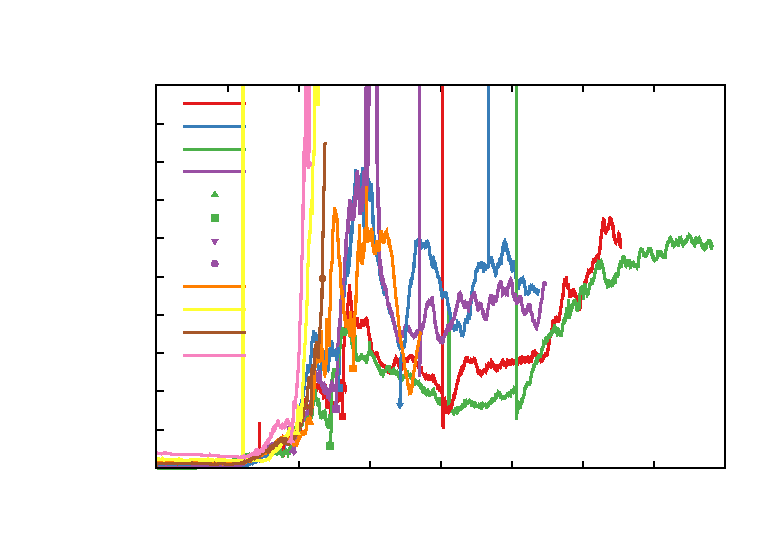
\includegraphics{images/combined-neutrino-luminosity}}%
    \gplfronttext
  \end{picture}%
\endgroup

	\caption[]{
		\textbf{TODO}
	}
	\label{fig:neutrinoluminosity}
\end{figure}

%\begin{figure}
%	\centering
%	% GNUPLOT: LaTeX picture with Postscript
\begingroup
  \makeatletter
  \providecommand\color[2][]{%
    \GenericError{(gnuplot) \space\space\space\@spaces}{%
      Package color not loaded in conjunction with
      terminal option `colourtext'%
    }{See the gnuplot documentation for explanation.%
    }{Either use 'blacktext' in gnuplot or load the package
      color.sty in LaTeX.}%
    \renewcommand\color[2][]{}%
  }%
  \providecommand\includegraphics[2][]{%
    \GenericError{(gnuplot) \space\space\space\@spaces}{%
      Package graphicx or graphics not loaded%
    }{See the gnuplot documentation for explanation.%
    }{The gnuplot epslatex terminal needs graphicx.sty or graphics.sty.}%
    \renewcommand\includegraphics[2][]{}%
  }%
  \providecommand\rotatebox[2]{#2}%
  \@ifundefined{ifGPcolor}{%
    \newif\ifGPcolor
    \GPcolortrue
  }{}%
  \@ifundefined{ifGPblacktext}{%
    \newif\ifGPblacktext
    \GPblacktexttrue
  }{}%
  % define a \g@addto@macro without @ in the name:
  \let\gplgaddtomacro\g@addto@macro
  % define empty templates for all commands taking text:
  \gdef\gplbacktext{}%
  \gdef\gplfronttext{}%
  \makeatother
  \ifGPblacktext
    % no textcolor at all
    \def\colorrgb#1{}%
    \def\colorgray#1{}%
  \else
    % gray or color?
    \ifGPcolor
      \def\colorrgb#1{\color[rgb]{#1}}%
      \def\colorgray#1{\color[gray]{#1}}%
      \expandafter\def\csname LTw\endcsname{\color{white}}%
      \expandafter\def\csname LTb\endcsname{\color{black}}%
      \expandafter\def\csname LTa\endcsname{\color{black}}%
      \expandafter\def\csname LT0\endcsname{\color[rgb]{1,0,0}}%
      \expandafter\def\csname LT1\endcsname{\color[rgb]{0,1,0}}%
      \expandafter\def\csname LT2\endcsname{\color[rgb]{0,0,1}}%
      \expandafter\def\csname LT3\endcsname{\color[rgb]{1,0,1}}%
      \expandafter\def\csname LT4\endcsname{\color[rgb]{0,1,1}}%
      \expandafter\def\csname LT5\endcsname{\color[rgb]{1,1,0}}%
      \expandafter\def\csname LT6\endcsname{\color[rgb]{0,0,0}}%
      \expandafter\def\csname LT7\endcsname{\color[rgb]{1,0.3,0}}%
      \expandafter\def\csname LT8\endcsname{\color[rgb]{0.5,0.5,0.5}}%
    \else
      % gray
      \def\colorrgb#1{\color{black}}%
      \def\colorgray#1{\color[gray]{#1}}%
      \expandafter\def\csname LTw\endcsname{\color{white}}%
      \expandafter\def\csname LTb\endcsname{\color{black}}%
      \expandafter\def\csname LTa\endcsname{\color{black}}%
      \expandafter\def\csname LT0\endcsname{\color{black}}%
      \expandafter\def\csname LT1\endcsname{\color{black}}%
      \expandafter\def\csname LT2\endcsname{\color{black}}%
      \expandafter\def\csname LT3\endcsname{\color{black}}%
      \expandafter\def\csname LT4\endcsname{\color{black}}%
      \expandafter\def\csname LT5\endcsname{\color{black}}%
      \expandafter\def\csname LT6\endcsname{\color{black}}%
      \expandafter\def\csname LT7\endcsname{\color{black}}%
      \expandafter\def\csname LT8\endcsname{\color{black}}%
    \fi
  \fi
  \setlength{\unitlength}{0.0500bp}%
  \begin{picture}(7200.00,5040.00)%
    \gplgaddtomacro\gplbacktext{%
      \csname LTb\endcsname%
      \put(1078,704){\makebox(0,0)[r]{\strut{} 0}}%
      \put(1078,1112){\makebox(0,0)[r]{\strut{} 0.01}}%
      \put(1078,1521){\makebox(0,0)[r]{\strut{} 0.02}}%
      \put(1078,1929){\makebox(0,0)[r]{\strut{} 0.03}}%
      \put(1078,2337){\makebox(0,0)[r]{\strut{} 0.04}}%
      \put(1078,2746){\makebox(0,0)[r]{\strut{} 0.05}}%
      \put(1078,3154){\makebox(0,0)[r]{\strut{} 0.06}}%
      \put(1078,3562){\makebox(0,0)[r]{\strut{} 0.07}}%
      \put(1078,3971){\makebox(0,0)[r]{\strut{} 0.08}}%
      \put(1078,4379){\makebox(0,0)[r]{\strut{} 0.09}}%
      \put(1210,484){\makebox(0,0){\strut{} 0}}%
      \put(1909,484){\makebox(0,0){\strut{} 2}}%
      \put(2608,484){\makebox(0,0){\strut{} 4}}%
      \put(3307,484){\makebox(0,0){\strut{} 6}}%
      \put(4007,484){\makebox(0,0){\strut{} 8}}%
      \put(4706,484){\makebox(0,0){\strut{} 10}}%
      \put(5405,484){\makebox(0,0){\strut{} 12}}%
      \put(6104,484){\makebox(0,0){\strut{} 14}}%
      \put(6803,484){\makebox(0,0){\strut{} 16}}%
      \put(176,2541){\rotatebox{-270}{\makebox(0,0){\strut{}unbound mass ($M_{\odot}$)}}}%
      \put(4006,154){\makebox(0,0){\strut{}$t - t_{\rm plunge}$ (ms)}}%
      \put(4006,4709){\makebox(0,0){\strut{}Unbound mass in merger for hot Nuclear-theory EOSs}}%
    }%
    \gplgaddtomacro\gplfronttext{%
      \csname LTb\endcsname%
      \put(2197,4206){\makebox(0,0)[l]{\strut{}Hempel DD2 M=1.2}}%
      \csname LTb\endcsname%
      \put(2197,3986){\makebox(0,0)[l]{\strut{}Hempel DD2 M=1.4}}%
      \csname LTb\endcsname%
      \put(2197,3766){\makebox(0,0)[l]{\strut{}G. Shen FSU 2.1, M=1.2}}%
      \csname LTb\endcsname%
      \put(2197,3546){\makebox(0,0)[l]{\strut{}G. Shen FSU 2.1, M=1.4}}%
      \csname LTb\endcsname%
      \put(2197,3326){\makebox(0,0)[l]{\strut{}SettleDisk}}%
      \csname LTb\endcsname%
      \put(2197,3106){\makebox(0,0)[l]{\strut{}Derefinement 1}}%
      \csname LTb\endcsname%
      \put(2197,2886){\makebox(0,0)[l]{\strut{}Derefinement 2}}%
      \csname LTb\endcsname%
      \put(2197,2666){\makebox(0,0)[l]{\strut{}Adaptive JB}}%
      \csname LTb\endcsname%
      \put(2197,2446){\makebox(0,0)[l]{\strut{}SFHo M=1.2}}%
      \csname LTb\endcsname%
      \put(2197,2226){\makebox(0,0)[l]{\strut{}SFHo M=1.4}}%
      \csname LTb\endcsname%
      \put(2197,2006){\makebox(0,0)[l]{\strut{}SFHx M=1.2}}%
      \csname LTb\endcsname%
      \put(2197,1786){\makebox(0,0)[l]{\strut{}SFHx M=1.4}}%
    }%
    \gplbacktext
    \put(0,0){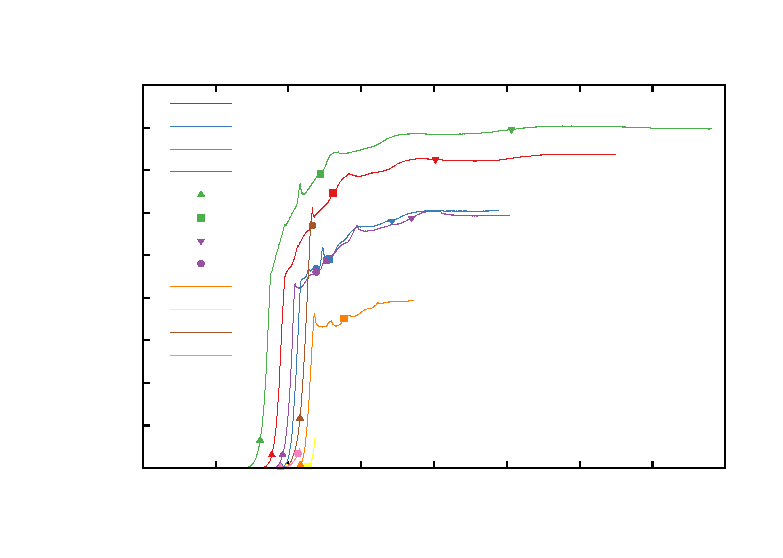
\includegraphics{images/combined-unbound-mass}}%
    \gplfronttext
  \end{picture}%
\endgroup

%	\caption[]{
%		\textbf{TODO}
%	}
%	\label{fig:unboundmass}
%\end{figure}
%
%\begin{figure}
%	\centering
%	% GNUPLOT: LaTeX picture with Postscript
\begingroup
  \makeatletter
  \providecommand\color[2][]{%
    \GenericError{(gnuplot) \space\space\space\@spaces}{%
      Package color not loaded in conjunction with
      terminal option `colourtext'%
    }{See the gnuplot documentation for explanation.%
    }{Either use 'blacktext' in gnuplot or load the package
      color.sty in LaTeX.}%
    \renewcommand\color[2][]{}%
  }%
  \providecommand\includegraphics[2][]{%
    \GenericError{(gnuplot) \space\space\space\@spaces}{%
      Package graphicx or graphics not loaded%
    }{See the gnuplot documentation for explanation.%
    }{The gnuplot epslatex terminal needs graphicx.sty or graphics.sty.}%
    \renewcommand\includegraphics[2][]{}%
  }%
  \providecommand\rotatebox[2]{#2}%
  \@ifundefined{ifGPcolor}{%
    \newif\ifGPcolor
    \GPcolortrue
  }{}%
  \@ifundefined{ifGPblacktext}{%
    \newif\ifGPblacktext
    \GPblacktexttrue
  }{}%
  % define a \g@addto@macro without @ in the name:
  \let\gplgaddtomacro\g@addto@macro
  % define empty templates for all commands taking text:
  \gdef\gplbacktext{}%
  \gdef\gplfronttext{}%
  \makeatother
  \ifGPblacktext
    % no textcolor at all
    \def\colorrgb#1{}%
    \def\colorgray#1{}%
  \else
    % gray or color?
    \ifGPcolor
      \def\colorrgb#1{\color[rgb]{#1}}%
      \def\colorgray#1{\color[gray]{#1}}%
      \expandafter\def\csname LTw\endcsname{\color{white}}%
      \expandafter\def\csname LTb\endcsname{\color{black}}%
      \expandafter\def\csname LTa\endcsname{\color{black}}%
      \expandafter\def\csname LT0\endcsname{\color[rgb]{1,0,0}}%
      \expandafter\def\csname LT1\endcsname{\color[rgb]{0,1,0}}%
      \expandafter\def\csname LT2\endcsname{\color[rgb]{0,0,1}}%
      \expandafter\def\csname LT3\endcsname{\color[rgb]{1,0,1}}%
      \expandafter\def\csname LT4\endcsname{\color[rgb]{0,1,1}}%
      \expandafter\def\csname LT5\endcsname{\color[rgb]{1,1,0}}%
      \expandafter\def\csname LT6\endcsname{\color[rgb]{0,0,0}}%
      \expandafter\def\csname LT7\endcsname{\color[rgb]{1,0.3,0}}%
      \expandafter\def\csname LT8\endcsname{\color[rgb]{0.5,0.5,0.5}}%
    \else
      % gray
      \def\colorrgb#1{\color{black}}%
      \def\colorgray#1{\color[gray]{#1}}%
      \expandafter\def\csname LTw\endcsname{\color{white}}%
      \expandafter\def\csname LTb\endcsname{\color{black}}%
      \expandafter\def\csname LTa\endcsname{\color{black}}%
      \expandafter\def\csname LT0\endcsname{\color{black}}%
      \expandafter\def\csname LT1\endcsname{\color{black}}%
      \expandafter\def\csname LT2\endcsname{\color{black}}%
      \expandafter\def\csname LT3\endcsname{\color{black}}%
      \expandafter\def\csname LT4\endcsname{\color{black}}%
      \expandafter\def\csname LT5\endcsname{\color{black}}%
      \expandafter\def\csname LT6\endcsname{\color{black}}%
      \expandafter\def\csname LT7\endcsname{\color{black}}%
      \expandafter\def\csname LT8\endcsname{\color{black}}%
    \fi
  \fi
  \setlength{\unitlength}{0.0500bp}%
  \begin{picture}(7200.00,5040.00)%
    \gplgaddtomacro\gplbacktext{%
      \csname LTb\endcsname%
      \put(1474,702){\makebox(0,0)[r]{\strut{} 0}}%
      \put(1474,1298){\makebox(0,0)[r]{\strut{} 2e+14}}%
      \put(1474,1893){\makebox(0,0)[r]{\strut{} 4e+14}}%
      \put(1474,2488){\makebox(0,0)[r]{\strut{} 6e+14}}%
      \put(1474,3084){\makebox(0,0)[r]{\strut{} 8e+14}}%
      \put(1474,3679){\makebox(0,0)[r]{\strut{} 1e+15}}%
      \put(1474,4275){\makebox(0,0)[r]{\strut{} 1.2e+15}}%
      \put(1606,484){\makebox(0,0){\strut{} 0}}%
      \put(2256,484){\makebox(0,0){\strut{} 2}}%
      \put(2905,484){\makebox(0,0){\strut{} 4}}%
      \put(3555,484){\makebox(0,0){\strut{} 6}}%
      \put(4205,484){\makebox(0,0){\strut{} 8}}%
      \put(4854,484){\makebox(0,0){\strut{} 10}}%
      \put(5504,484){\makebox(0,0){\strut{} 12}}%
      \put(6153,484){\makebox(0,0){\strut{} 14}}%
      \put(6803,484){\makebox(0,0){\strut{} 16}}%
      \put(176,2541){\rotatebox{-270}{\makebox(0,0){\strut{}$\rho_0^{\rm max}$ (${\rm g\,cm}^{-3}$)}}}%
      \put(4204,154){\makebox(0,0){\strut{}$t - t_{\rm plunge}$ (ms)}}%
      \put(4204,4709){\makebox(0,0){\strut{}Densest point in plunge-merger for hot Nuclear-theory EOSs}}%
    }%
    \gplgaddtomacro\gplfronttext{%
      \csname LTb\endcsname%
      \put(5816,4206){\makebox(0,0)[r]{\strut{}Hempel DD2 M=1.2}}%
      \csname LTb\endcsname%
      \put(5816,3986){\makebox(0,0)[r]{\strut{}Hempel DD2 M=1.4}}%
      \csname LTb\endcsname%
      \put(5816,3766){\makebox(0,0)[r]{\strut{}G. Shen FSU 2.1, M=1.2}}%
      \csname LTb\endcsname%
      \put(5816,3546){\makebox(0,0)[r]{\strut{}G. Shen FSU 2.1, M=1.4}}%
      \csname LTb\endcsname%
      \put(5816,3326){\makebox(0,0)[r]{\strut{}SettleDisk}}%
      \csname LTb\endcsname%
      \put(5816,3106){\makebox(0,0)[r]{\strut{}Derefinement 1}}%
      \csname LTb\endcsname%
      \put(5816,2886){\makebox(0,0)[r]{\strut{}Derefinement 2}}%
      \csname LTb\endcsname%
      \put(5816,2666){\makebox(0,0)[r]{\strut{}Adaptive JB}}%
      \csname LTb\endcsname%
      \put(5816,2446){\makebox(0,0)[r]{\strut{}SFHo M=1.2}}%
      \csname LTb\endcsname%
      \put(5816,2226){\makebox(0,0)[r]{\strut{}SFHo M=1.4}}%
      \csname LTb\endcsname%
      \put(5816,2006){\makebox(0,0)[r]{\strut{}SFHx M=1.2}}%
      \csname LTb\endcsname%
      \put(5816,1786){\makebox(0,0)[r]{\strut{}SFHx M=1.4}}%
    }%
    \gplbacktext
    \put(0,0){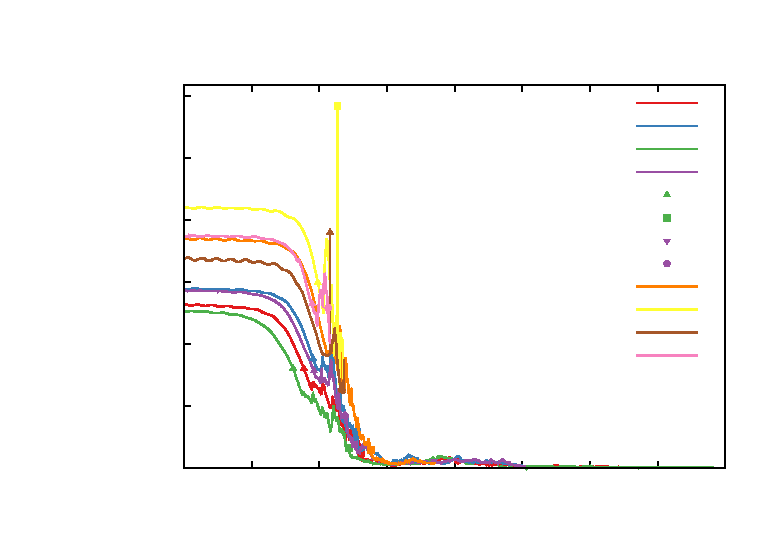
\includegraphics{images/combined-densest-point}}%
    \gplfronttext
  \end{picture}%
\endgroup

%	\caption[]{
%		\textbf{TODO}
%	}
%	\label{fig:densestpoint}
%\end{figure}
%
%\begin{figure}
%	\centering
%	% GNUPLOT: LaTeX picture with Postscript
\begingroup
  \makeatletter
  \providecommand\color[2][]{%
    \GenericError{(gnuplot) \space\space\space\@spaces}{%
      Package color not loaded in conjunction with
      terminal option `colourtext'%
    }{See the gnuplot documentation for explanation.%
    }{Either use 'blacktext' in gnuplot or load the package
      color.sty in LaTeX.}%
    \renewcommand\color[2][]{}%
  }%
  \providecommand\includegraphics[2][]{%
    \GenericError{(gnuplot) \space\space\space\@spaces}{%
      Package graphicx or graphics not loaded%
    }{See the gnuplot documentation for explanation.%
    }{The gnuplot epslatex terminal needs graphicx.sty or graphics.sty.}%
    \renewcommand\includegraphics[2][]{}%
  }%
  \providecommand\rotatebox[2]{#2}%
  \@ifundefined{ifGPcolor}{%
    \newif\ifGPcolor
    \GPcolortrue
  }{}%
  \@ifundefined{ifGPblacktext}{%
    \newif\ifGPblacktext
    \GPblacktexttrue
  }{}%
  % define a \g@addto@macro without @ in the name:
  \let\gplgaddtomacro\g@addto@macro
  % define empty templates for all commands taking text:
  \gdef\gplbacktext{}%
  \gdef\gplfronttext{}%
  \makeatother
  \ifGPblacktext
    % no textcolor at all
    \def\colorrgb#1{}%
    \def\colorgray#1{}%
  \else
    % gray or color?
    \ifGPcolor
      \def\colorrgb#1{\color[rgb]{#1}}%
      \def\colorgray#1{\color[gray]{#1}}%
      \expandafter\def\csname LTw\endcsname{\color{white}}%
      \expandafter\def\csname LTb\endcsname{\color{black}}%
      \expandafter\def\csname LTa\endcsname{\color{black}}%
      \expandafter\def\csname LT0\endcsname{\color[rgb]{1,0,0}}%
      \expandafter\def\csname LT1\endcsname{\color[rgb]{0,1,0}}%
      \expandafter\def\csname LT2\endcsname{\color[rgb]{0,0,1}}%
      \expandafter\def\csname LT3\endcsname{\color[rgb]{1,0,1}}%
      \expandafter\def\csname LT4\endcsname{\color[rgb]{0,1,1}}%
      \expandafter\def\csname LT5\endcsname{\color[rgb]{1,1,0}}%
      \expandafter\def\csname LT6\endcsname{\color[rgb]{0,0,0}}%
      \expandafter\def\csname LT7\endcsname{\color[rgb]{1,0.3,0}}%
      \expandafter\def\csname LT8\endcsname{\color[rgb]{0.5,0.5,0.5}}%
    \else
      % gray
      \def\colorrgb#1{\color{black}}%
      \def\colorgray#1{\color[gray]{#1}}%
      \expandafter\def\csname LTw\endcsname{\color{white}}%
      \expandafter\def\csname LTb\endcsname{\color{black}}%
      \expandafter\def\csname LTa\endcsname{\color{black}}%
      \expandafter\def\csname LT0\endcsname{\color{black}}%
      \expandafter\def\csname LT1\endcsname{\color{black}}%
      \expandafter\def\csname LT2\endcsname{\color{black}}%
      \expandafter\def\csname LT3\endcsname{\color{black}}%
      \expandafter\def\csname LT4\endcsname{\color{black}}%
      \expandafter\def\csname LT5\endcsname{\color{black}}%
      \expandafter\def\csname LT6\endcsname{\color{black}}%
      \expandafter\def\csname LT7\endcsname{\color{black}}%
      \expandafter\def\csname LT8\endcsname{\color{black}}%
    \fi
  \fi
  \setlength{\unitlength}{0.0500bp}%
  \begin{picture}(7200.00,5040.00)%
    \gplgaddtomacro\gplbacktext{%
      \csname LTb\endcsname%
      \put(1078,704){\makebox(0,0)[r]{\strut{} 0.01}}%
      \put(1078,1156){\makebox(0,0)[r]{\strut{} 0.02}}%
      \put(1078,1609){\makebox(0,0)[r]{\strut{} 0.03}}%
      \put(1078,2061){\makebox(0,0)[r]{\strut{} 0.04}}%
      \put(1078,2513){\makebox(0,0)[r]{\strut{} 0.05}}%
      \put(1078,2966){\makebox(0,0)[r]{\strut{} 0.06}}%
      \put(1078,3418){\makebox(0,0)[r]{\strut{} 0.07}}%
      \put(1078,3870){\makebox(0,0)[r]{\strut{} 0.08}}%
      \put(1078,4323){\makebox(0,0)[r]{\strut{} 0.09}}%
      \put(1078,4775){\makebox(0,0)[r]{\strut{} 0.1}}%
      \put(1210,484){\makebox(0,0){\strut{} 0}}%
      \put(2009,484){\makebox(0,0){\strut{} 2}}%
      \put(2808,484){\makebox(0,0){\strut{} 4}}%
      \put(3607,484){\makebox(0,0){\strut{} 6}}%
      \put(4406,484){\makebox(0,0){\strut{} 8}}%
      \put(5205,484){\makebox(0,0){\strut{} 10}}%
      \put(6004,484){\makebox(0,0){\strut{} 12}}%
      \put(6803,484){\makebox(0,0){\strut{} 14}}%
      \put(176,2739){\rotatebox{-270}{\makebox(0,0){\strut{}$\langle Y_e \rangle$}}}%
      \put(4006,154){\makebox(0,0){\strut{}$t - t_{\rm settledisk}$ (ms)}}%
    }%
    \gplgaddtomacro\gplfronttext{%
      \csname LTb\endcsname%
      \put(5816,4602){\makebox(0,0)[r]{\strut{}Hempel DD2 M=1.2}}%
      \csname LTb\endcsname%
      \put(5816,4382){\makebox(0,0)[r]{\strut{}Hempel DD2 M=1.4}}%
      \csname LTb\endcsname%
      \put(5816,4162){\makebox(0,0)[r]{\strut{}G. Shen FSU 2.1, M=1.2}}%
      \csname LTb\endcsname%
      \put(5816,3942){\makebox(0,0)[r]{\strut{}G. Shen FSU 2.1, M=1.4}}%
      \csname LTb\endcsname%
      \put(5816,3722){\makebox(0,0)[r]{\strut{}Derefinement 1}}%
      \csname LTb\endcsname%
      \put(5816,3502){\makebox(0,0)[r]{\strut{}Derefinement 2}}%
      \csname LTb\endcsname%
      \put(5816,3282){\makebox(0,0)[r]{\strut{}Adaptive JB}}%
      \csname LTb\endcsname%
      \put(5816,3062){\makebox(0,0)[r]{\strut{}SFHo M=1.2}}%
      \csname LTb\endcsname%
      \put(5816,2842){\makebox(0,0)[r]{\strut{}SFHo M=1.4}}%
      \csname LTb\endcsname%
      \put(5816,2622){\makebox(0,0)[r]{\strut{}SFHx M=1.2}}%
      \csname LTb\endcsname%
      \put(5816,2402){\makebox(0,0)[r]{\strut{}SFHx M=1.4}}%
    }%
    \gplbacktext
    \put(0,0){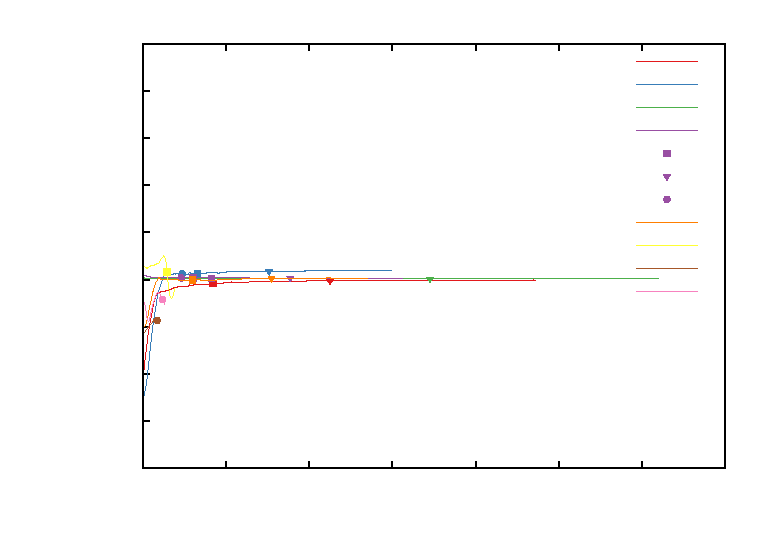
\includegraphics{images/unbound-ye-sd}}%
    \gplfronttext
  \end{picture}%
\endgroup

%	\caption[]{
%		\textbf{TODO}
%	}
%	\label{fig:unboundYe}
%\end{figure}



\begin{figure}
	\centering
	\begin{subfigure}[b]{0.475\textwidth}
		\centering
		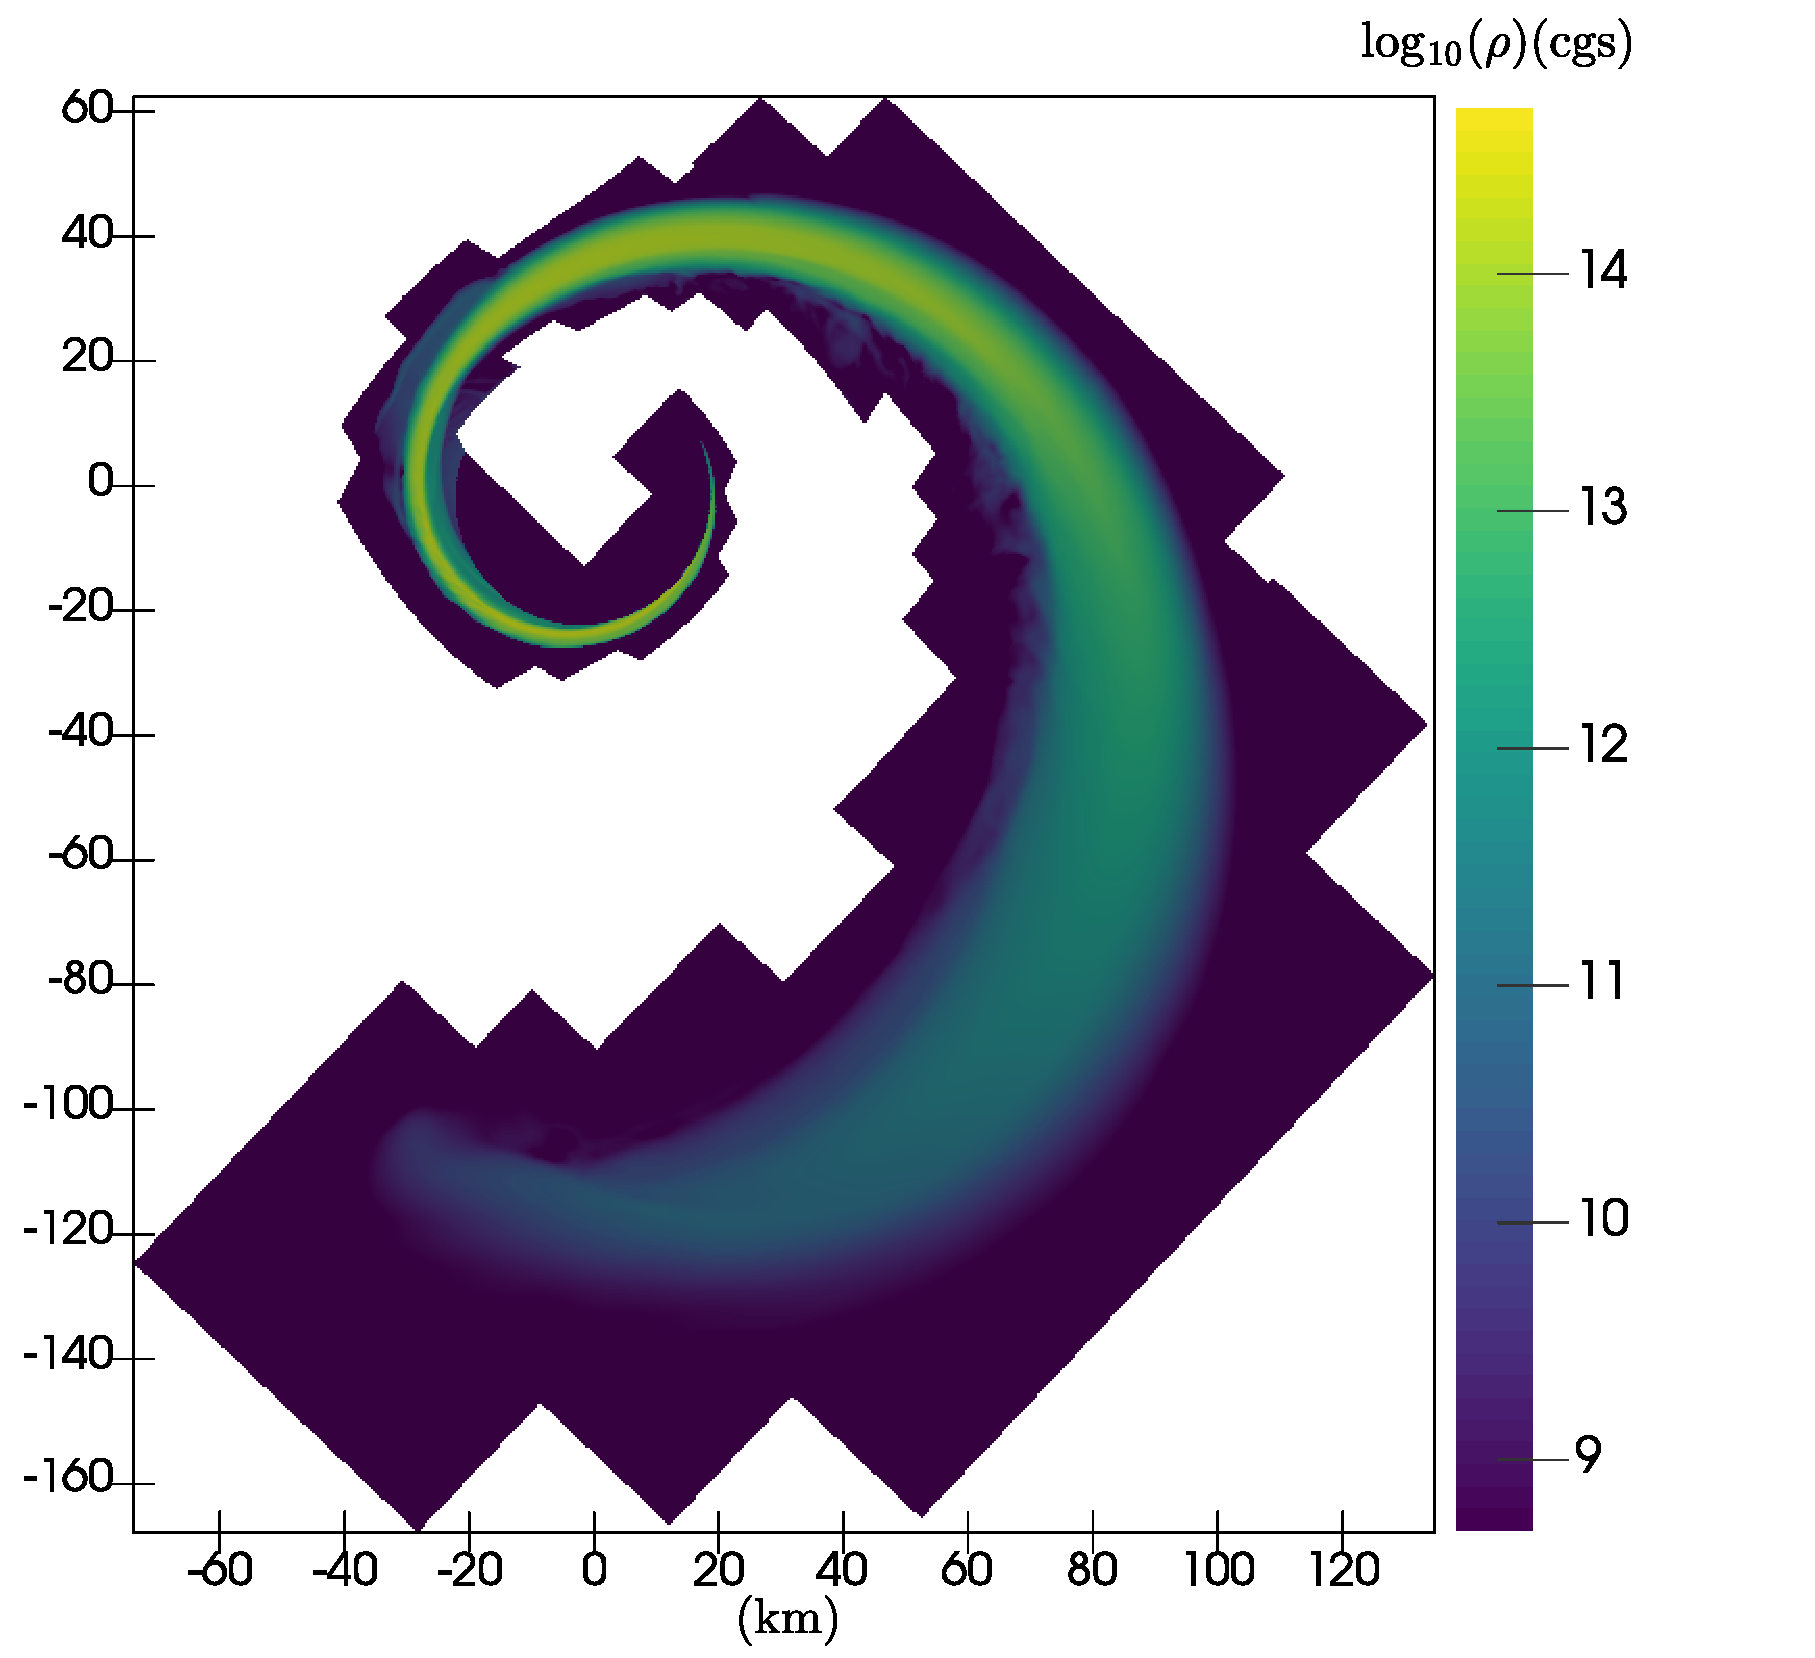
\includegraphics[width=1.0\linewidth]{images/rho_DD2_M12-merger-inertial}
		\label{fig:rho_M12_DD2}
	\end{subfigure}
	\begin{subfigure}[b]{0.475\textwidth}
		\centering
		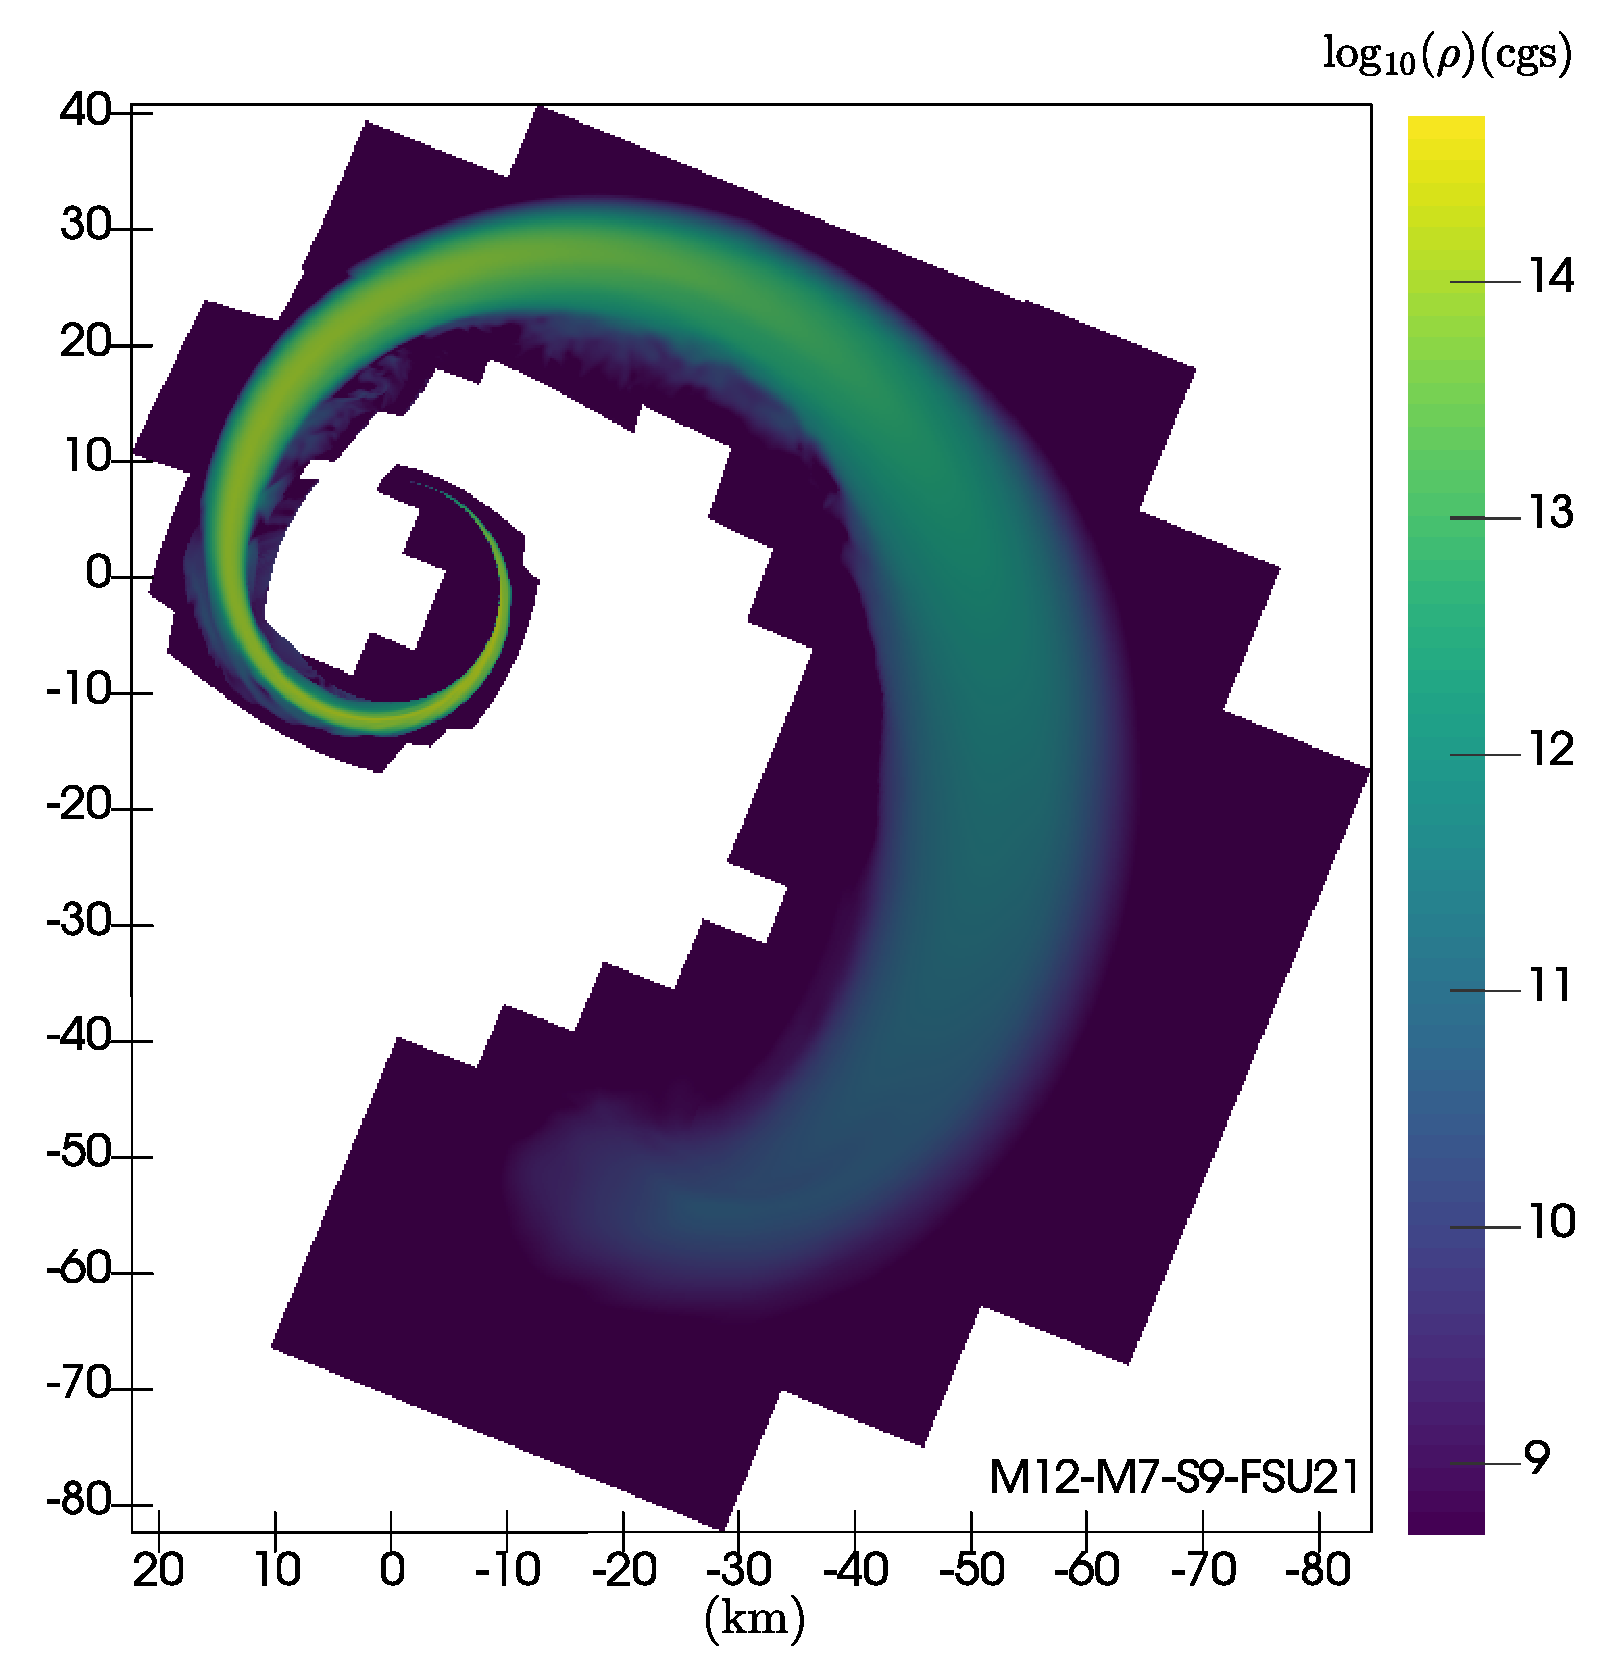
\includegraphics[width=\linewidth]{images/rho_FSU21_M12-merger-inertial}
		\label{fig:rho_M12_FSU21}
	\centering
	\end{subfigure}
	\begin{subfigure}[b]{0.475\textwidth}
		\centering
		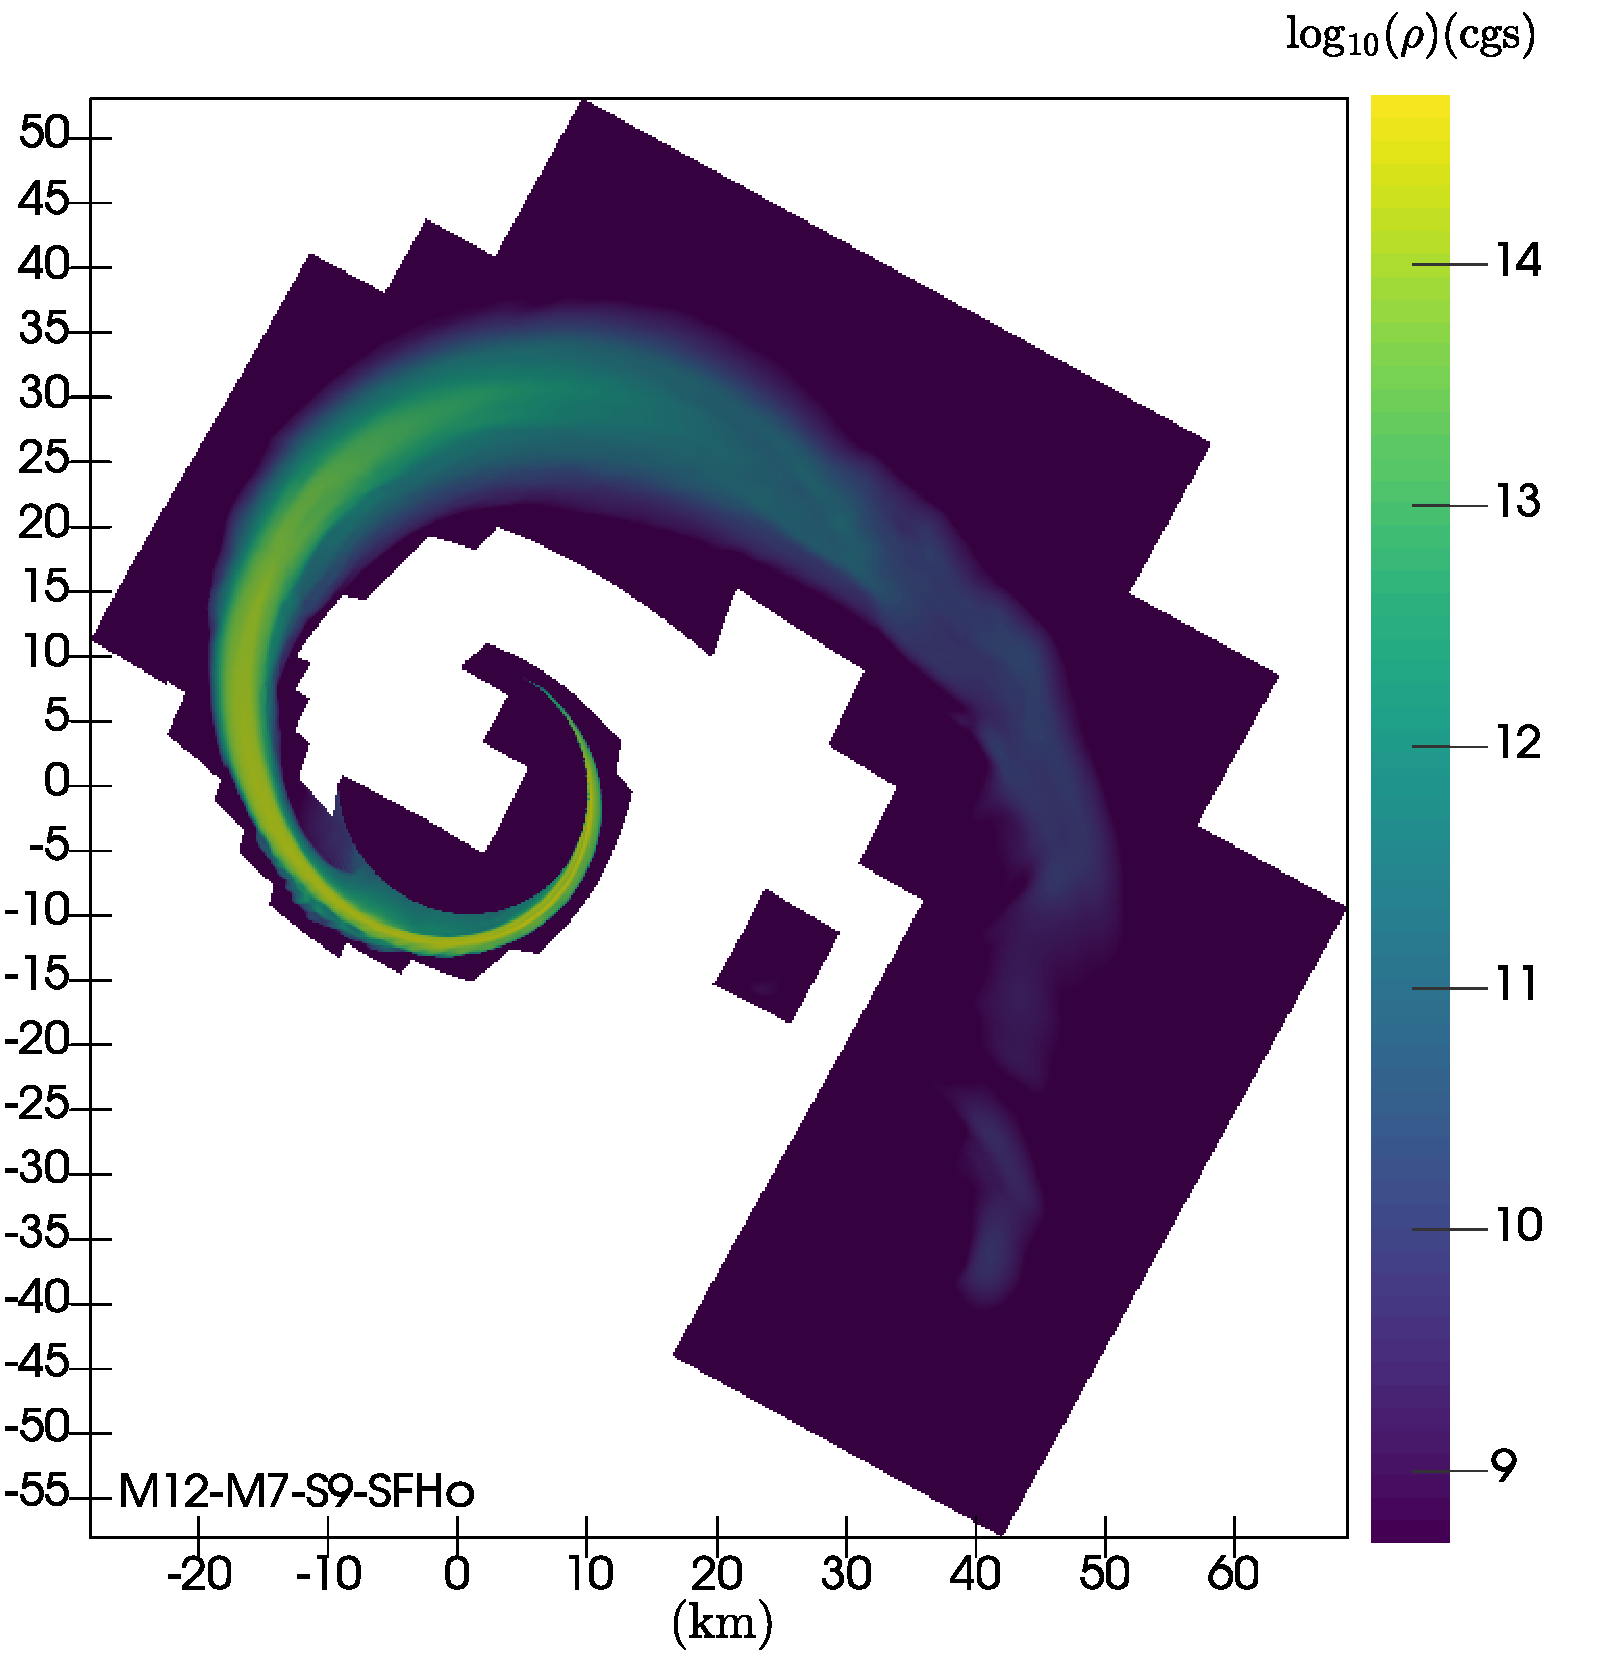
\includegraphics[width=\linewidth]{images/rho_SFHo_M12-merger-inertial}
		\label{fig:rho_M12_SFHo}
	\end{subfigure}
	\begin{subfigure}[b]{0.475\textwidth}
		\centering
		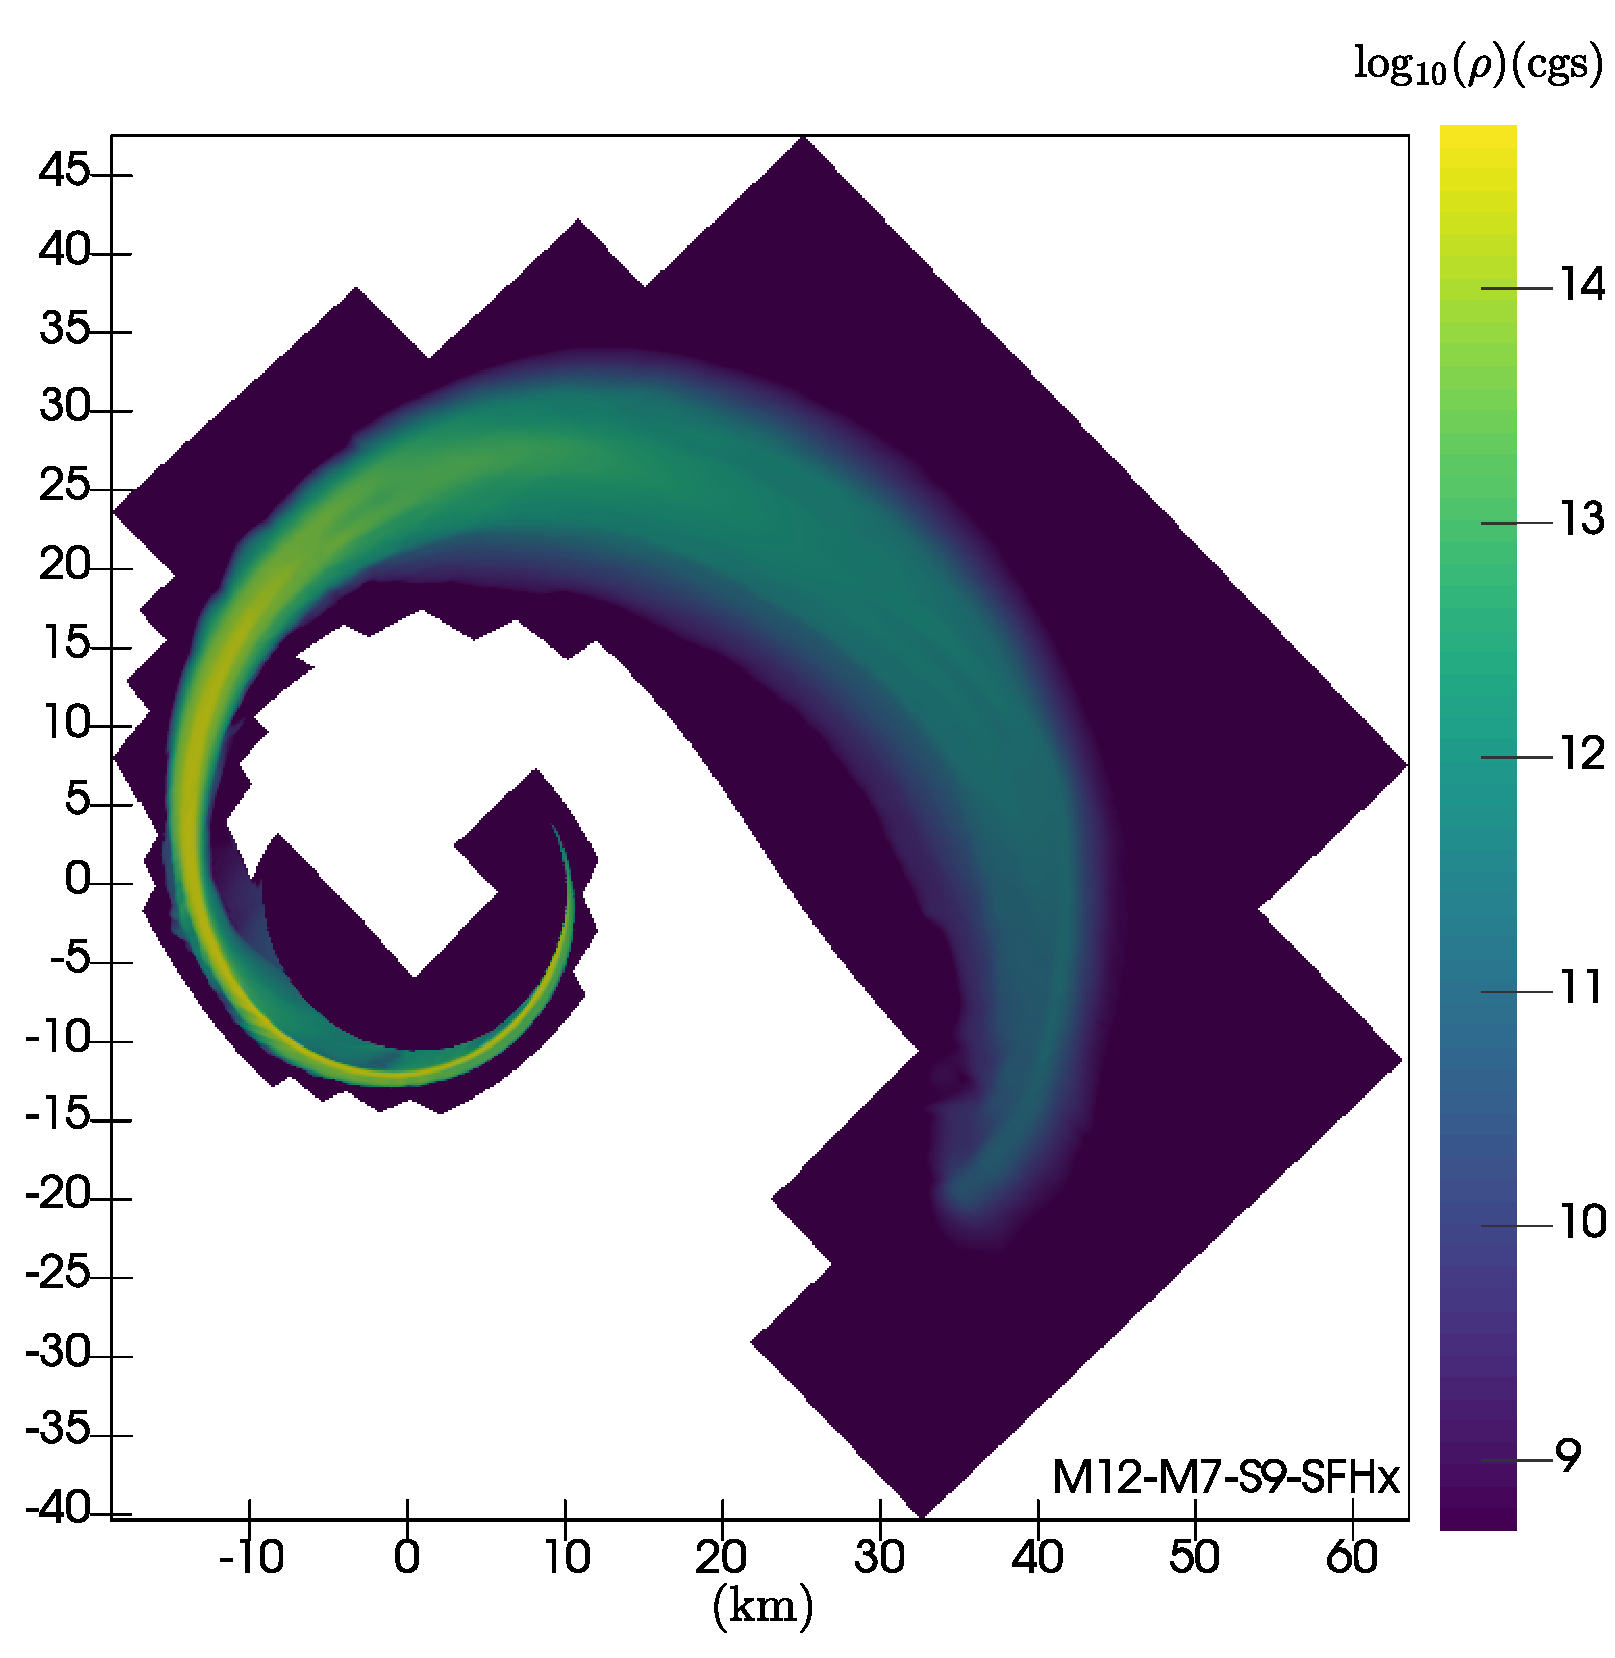
\includegraphics[width=\linewidth]{images/rho_SFHx_M12-merger-inertial}
		\label{fig:rho_M12_SFHx}
	\end{subfigure}
	\caption[Density profiles on equatorial plane for $1.2 M_{\odot}$ models]{
		Baryon density profiles on the equatorial plane for $M_{\rm NS} = 1.2 M_{\odot}$ models when $50\%$ of the neutron star material has been accreted onto the black hole.
		\textit{Top left:} Model M12-M7-S9-DD2.
		\textit{Top right:} Model M12-M7-S9-FSU21.
		\textit{Bottom left:} Model M12-M7-S9-SFHo.
		\textit{Bottom right:} Model M12-M7-S9-SFHx.
		White regions are not covered by the finite volume grid, while some fluid subdomains overlap the excised region of the black hole which can be seen near the interface of inflowing matter and the horizon.  We bracket the baryon density between $\sym \rho_{\rm FMR}$ and the fiducial density, $10^{14.7} {\rm g\,cm^{-3}}$. Note the distortion (and rotation) of the finite volume subdomain boundaries in the finest, innermost level, since the fluid is evolved in the coordinates of the (non-rotating) pseudo-spectral grid and we are viewing the systems in the inertial frame.  Also note the difference in length scales between models at merger time.
	}
	\label{fig:rho_M12}
\end{figure}


\begin{figure*}
	\centering
	\begin{subfigure}[b]{0.475\textwidth}
		\centering
		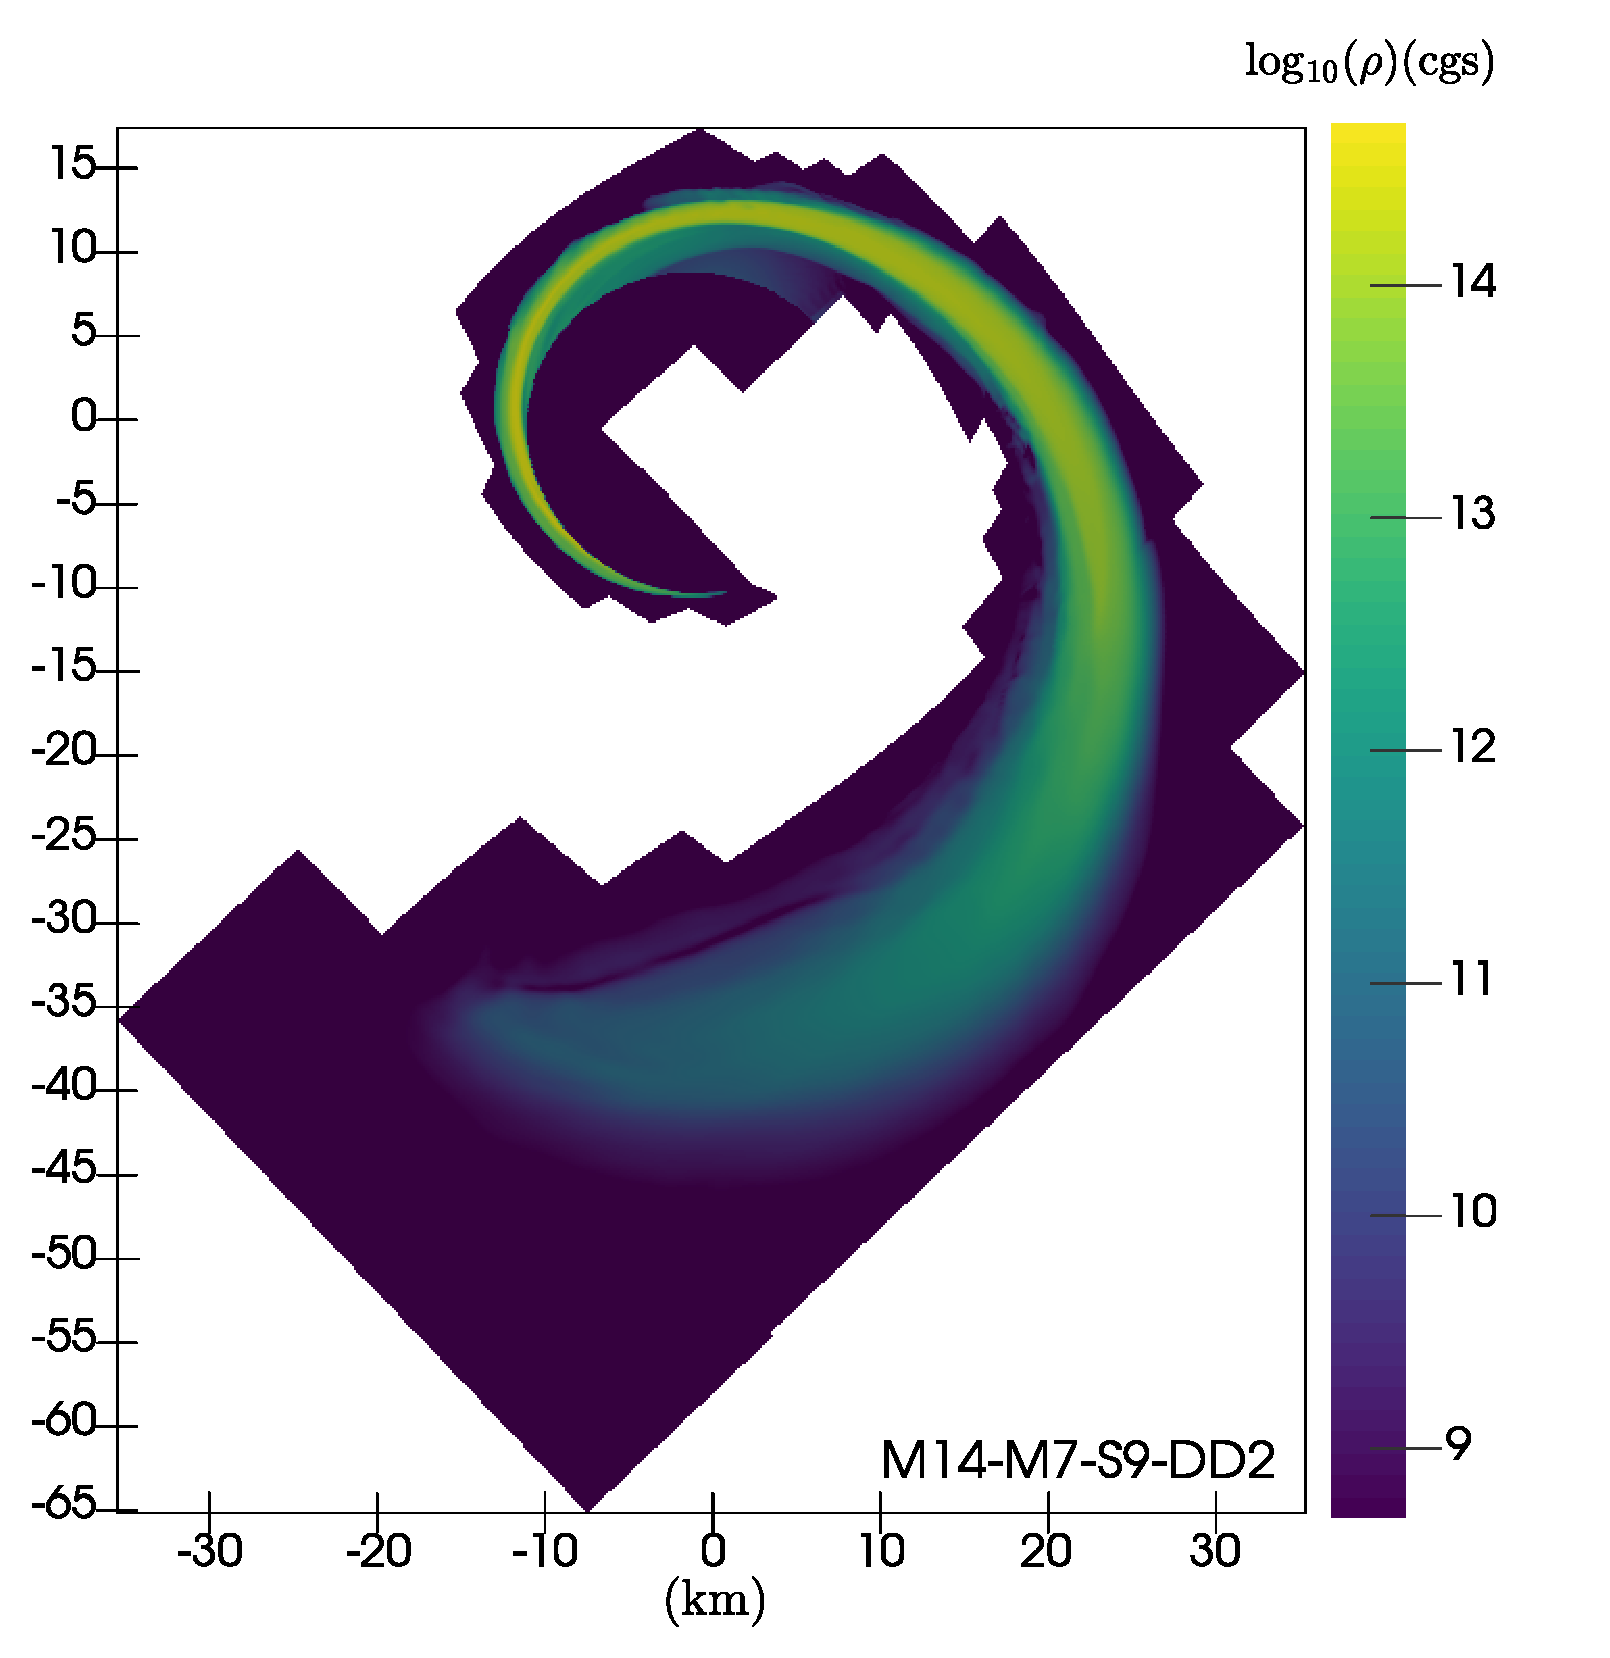
\includegraphics[width=1.0\linewidth]{images/rho_DD2_M14-merger-inertial}
		\label{fig:rho_M14_DD2}
	\end{subfigure}
	\begin{subfigure}[b]{0.475\textwidth}
		\centering
		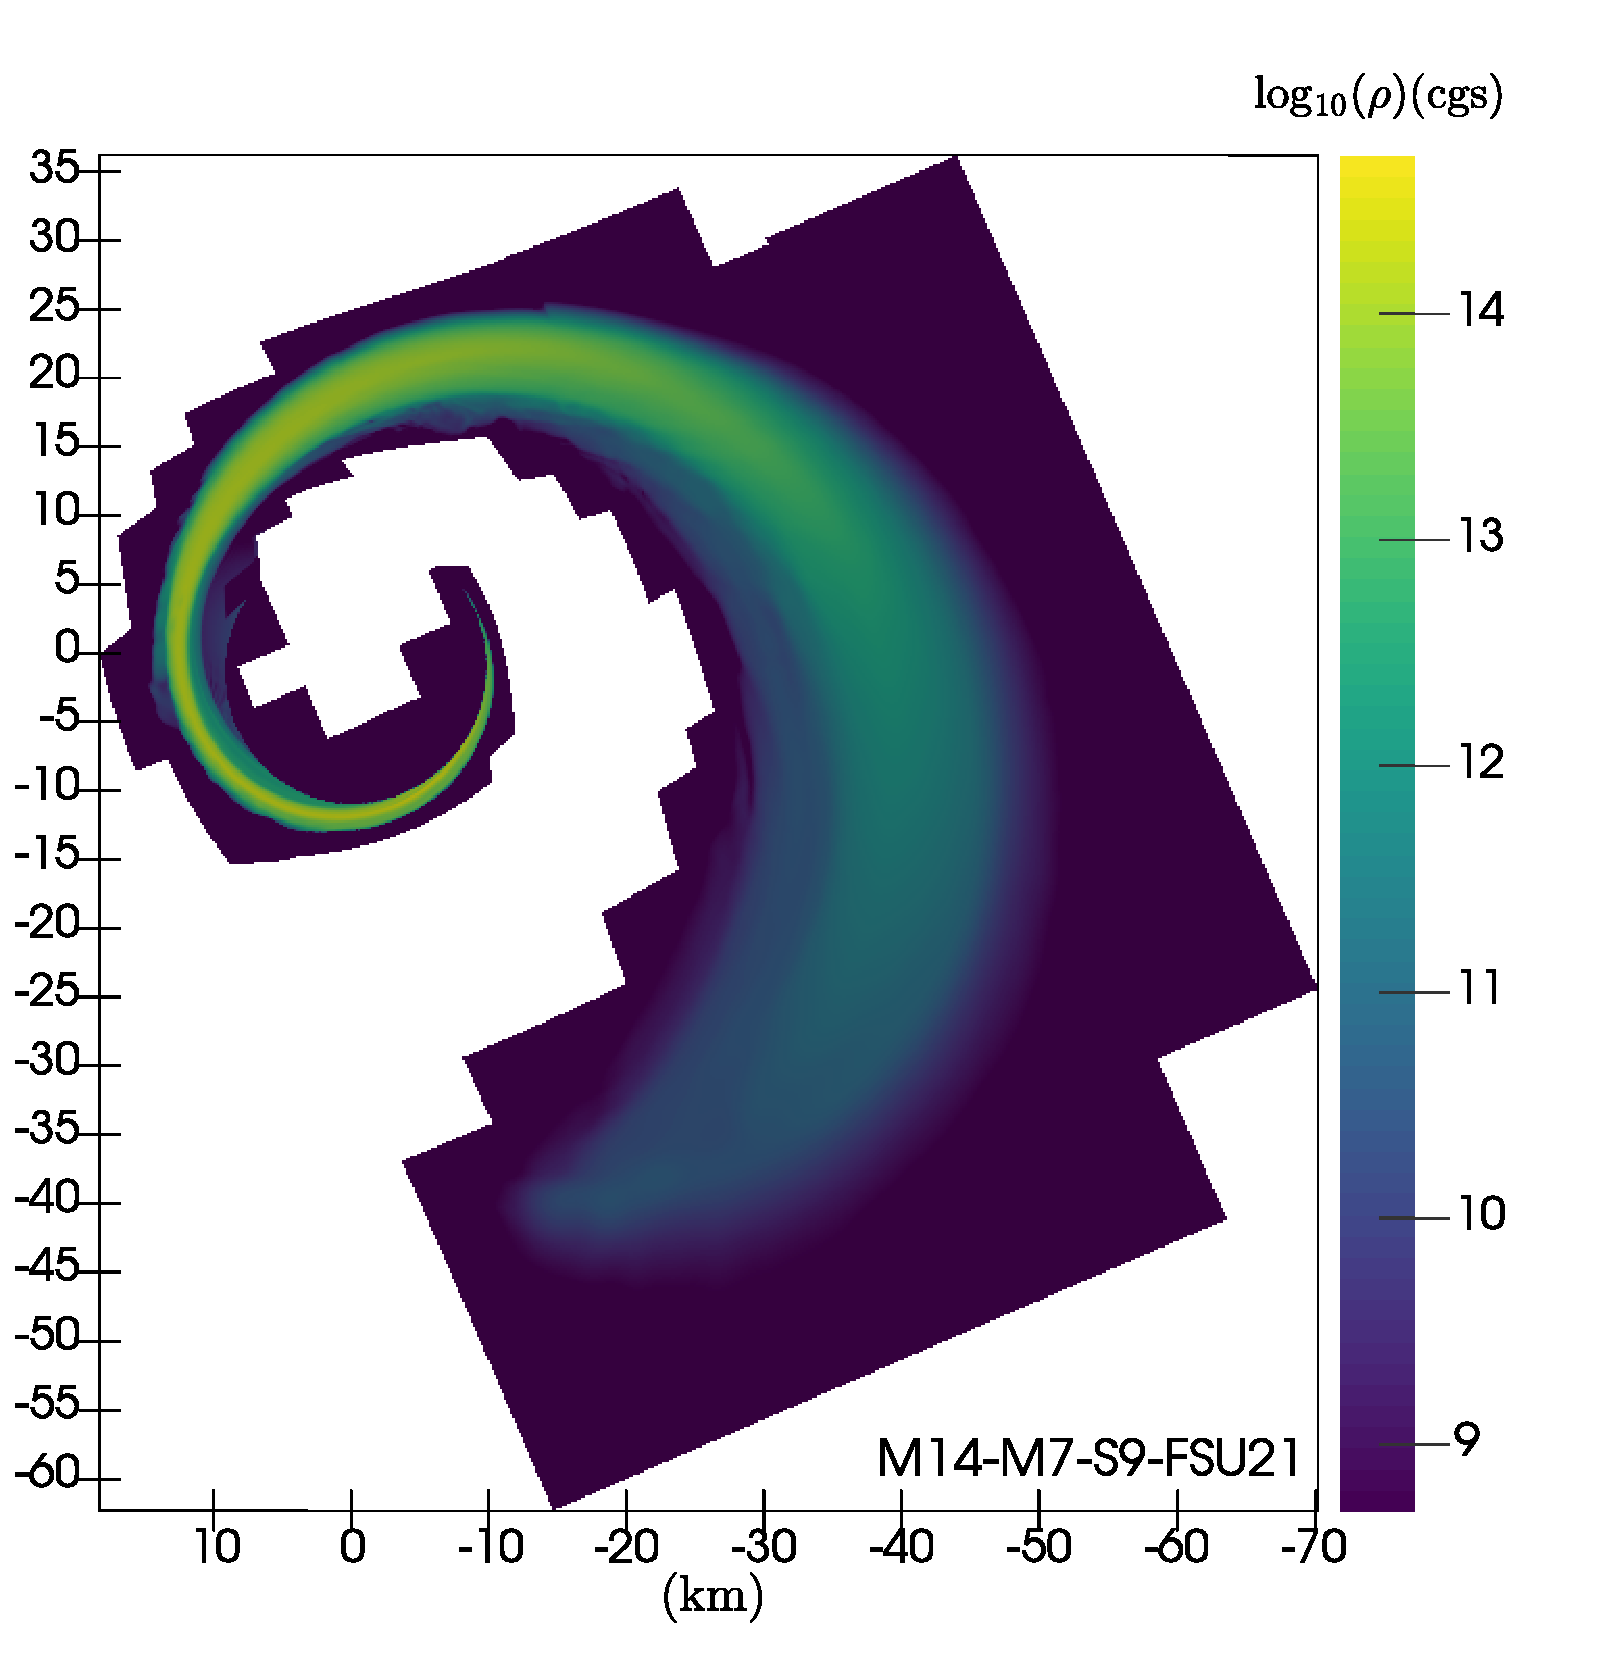
\includegraphics[width=\linewidth]{images/rho_FSU21_M14-merger-inertial}
		\label{fig:rho_M14_FSU21}
		\centering
	\end{subfigure}
	\caption[Density profiles on equatorial plane for $1.4 M_{\odot}$ models]{
	Baryon density profiles on the equatorial plane for $M_{\rm NS} = 1.4 M_{\odot}$ models when $50\%$ of the neutron star material has been accreted onto the black hole.
	\textit{Left:} Model M14-M7-S9-DD2.
	\textit{Right:} Model M14-M7-S9-FSU21.
	To add to the caption in Figure \ref{fig:rho_M12}, we note that the FSU2.1 profiles are represented with a $90^{\circ}$ counterclockwise rotation in the inertial frame.  This is done for sake of maintaining a similar aspect ratio to the others.  Note that FSU2.1 had the fewest number of orbits in our simulations (see Table \ref{tab:id}). 
	}
	\label{fig:rho_M14}
\end{figure*}